\section{Constructing Ladder Operator Block-Encodings}
\label{sec:ladder-op-oracles}

In this work, we focus on generating block-encodings for second-quantized Hamiltonians that include both fermionic and bosonic ladder operators.
In the previous sections, we discussed different methods to block-encode operators that are described as a product or linear combination of other operators.
In this section, we provide a framework for efficiently block-encoding individual ladder operators, products of ladder operators, and particular linear combinations of ladder operators.
We choose to explicitly include control qubits in our constructions since most use-cases of block-encodings require them to be controlled and controlling operations typically increases the cost of the operation.

\subsection{Encoding}
\label{subsec:encoding}

The encoding that is used for the occupation of the fermionic modes is identical to the Jordan-Wigner encoding \cite{jordan-wigner}.
The map between a Fock state to a qubit state is given as 
\begin{equation}
    \ket{n_{I_b}, \dots, n_{1_b}, n_{0_b}} \rightarrow \ket{q_{I_b}, \dots, q_{1_b}, q_{0_b}}
\end{equation}
where $n_{i_b} = q_{i_b} \in [0, 1]$ depending on if mode $i$ is occupied ($\ket{1}$) or unoccupied ($\ket{0}$).
The number of qubits required for the fermionic system is equal to the number of fermionic modes.

The encoding scheme for bosons must allow for occupancies in the range $[0, \Omega]$ due to the absence of the Pauli exclusion principle.
We choose to represent store the occupancy of a bosonic mode in binary notation: 
\begin{equation}
    \ket{n_{i_a}} \rightarrow \ket{b_j, b_{j-1}, ..., b_0}
\end{equation}
where $j$ runs from $0$ to $\lceil \log_2{\Omega} \rceil - 1$ and the values of $b_j$ are given by the binary representation of $n_{i_a}$.
This is identical to the encoding used in \cite{rhodes2024exponential}. \ws{check citation}

Storing the occupation of each bosonic mode requires $\lceil \log_2{\Omega} \rceil$ qubits if we assume that the maximum bosonic occupation is the same for each bosonic mode.
This choice of the maximum bosonic occupation being constant for all bosonic modes is not a restriction of the methods presented in this work, but is chosen for simplicity. 
With this choice, the number of qubits required for the bosonic subsystem is: $Q_{\psi_a} = I_a \lceil \log_2{\Omega} \rceil$.

\subsection{Fermionic Ladder Operators}
\label{subsec:fermionic-be}

Here, we aim to define a family of unitaries ($\{U_{b^\dagger_j}, U_{b_j}\}$) that generate block-encodings of the associated fermionic creation ($b_j^\dagger$) and annihilation ($b_j$) operators.
As these are block-encodings of non-unitary operators, we define the associated unitary operators to be of the form of Eq. \ref{eq:general-block-encoding}:
\begin{equation}
    U_{b^\dagger_j} \ket{\psi} \ket{0}_\text{anc} = b^\dagger_j \ket{\psi}\ket{0}_\text{anc} + \beta_\psi \ket{\perp}
\end{equation}
No rescaling factor is needed for these operators since the fermionic ladder operators have spectral norm of $1$.

The definition of the fermionic creation operator (Eq. \ref{eq:fermionic-creation}) creates two implications.
If the mode is unoccupied, then the mode should become occupied and a sign should be applied based on the occupancy of the preceeding fermionic modes.
If the mode is occupied, then state should be zeroed-out. 
Therefore, the action of our unitary will be dependent on the occupation of the fermionic mode:
\begin{equation}
    U_{b^\dagger_j} \ket{\psi_j} \ket{0}_\text{anc} =
    \begin{cases} 
        \ket{1} \ket{0}_\text{anc} & \text{when $\ket{\psi_j}$ is $\ket{0}$} \\
        \ket{\perp} & \text{when $\ket{\psi_j}$ is $\ket{1}$} \\
    \end{cases}
\end{equation}
where the sign flip caused by the occupation of the preceeding modes is omitted for brevity, but is assumed throughout the remainder of this section.

\begin{figure}[h]
    \mbox{
        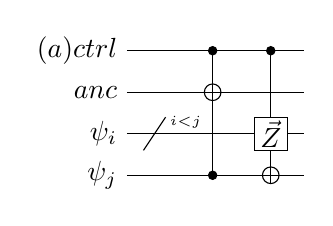
\begin{tikzpicture}[scale=1.000000,x=1pt,y=1pt]
\filldraw[color=white] (0.000000, -7.500000) rectangle (64.000000, 52.500000);
% Drawing wires
% Line 1: ctrl W \text{(a) }ctrl
\draw[color=black] (0.000000,45.000000) -- (64.000000,45.000000);
\draw[color=black] (0.000000,45.000000) node[left] {$\text{(a) }ctrl$};
% Line 2: anc W anc
\draw[color=black] (0.000000,30.000000) -- (64.000000,30.000000);
\draw[color=black] (0.000000,30.000000) node[left] {$anc$};
% Line 3: i W \psi_i
\draw[color=black] (0.000000,15.000000) -- (64.000000,15.000000);
\draw[color=black] (0.000000,15.000000) node[left] {$\psi_i$};
% Line 4: j W \psi_j
\draw[color=black] (0.000000,0.000000) -- (64.000000,0.000000);
\draw[color=black] (0.000000,0.000000) node[left] {$\psi_j$};
% Done with wires; drawing gates
% Line 6: i / ^{i<j}
\draw (6.000000, 9.000000) -- (14.000000, 21.000000);
\draw (12.000000, 18.000000) node[right] {$\scriptstyle{^{i<j}}$};
% Line 7: ctrl anc i j LABEL width=-10
% Line 8: ctrl j +anc
\draw (31.000000,45.000000) -- (31.000000,0.000000);
\filldraw (31.000000, 45.000000) circle(1.500000pt);
\filldraw (31.000000, 0.000000) circle(1.500000pt);
\begin{scope}
\draw[fill=white] (31.000000, 30.000000) circle(3.000000pt);
\clip (31.000000, 30.000000) circle(3.000000pt);
\draw (28.000000, 30.000000) -- (34.000000, 30.000000);
\draw (31.000000, 27.000000) -- (31.000000, 33.000000);
\end{scope}
% Line 10: i G $\vec{Z}$ ctrl +j
\draw (52.000000,45.000000) -- (52.000000,0.000000);
\begin{scope}
\draw[fill=white] (52.000000, 15.000000) +(-45.000000:8.485281pt and 8.485281pt) -- +(45.000000:8.485281pt and 8.485281pt) -- +(135.000000:8.485281pt and 8.485281pt) -- +(225.000000:8.485281pt and 8.485281pt) -- cycle;
\clip (52.000000, 15.000000) +(-45.000000:8.485281pt and 8.485281pt) -- +(45.000000:8.485281pt and 8.485281pt) -- +(135.000000:8.485281pt and 8.485281pt) -- +(225.000000:8.485281pt and 8.485281pt) -- cycle;
\draw (52.000000, 15.000000) node {$\vec{Z}$};
\end{scope}
\filldraw (52.000000, 45.000000) circle(1.500000pt);
\begin{scope}
\draw[fill=white] (52.000000, 0.000000) circle(3.000000pt);
\clip (52.000000, 0.000000) circle(3.000000pt);
\draw (49.000000, 0.000000) -- (55.000000, 0.000000);
\draw (52.000000, -3.000000) -- (52.000000, 3.000000);
\end{scope}
% Done with gates; drawing ending labels
% Done with ending labels; drawing cut lines and comments
% Done with comments
\end{tikzpicture}

        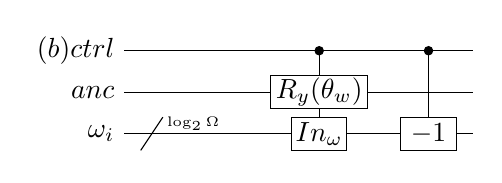
\begin{tikzpicture}[scale=1.000000,x=1pt,y=1pt]
\filldraw[color=white] (0.000000, -7.500000) rectangle (126.000000, 37.500000);
% Drawing wires
% Line 1: ctrl W \text{(b) }ctrl
\draw[color=black] (0.000000,30.000000) -- (126.000000,30.000000);
\draw[color=black] (0.000000,30.000000) node[left] {$\text{(b) }ctrl$};
% Line 2: anc W anc
\draw[color=black] (0.000000,15.000000) -- (126.000000,15.000000);
\draw[color=black] (0.000000,15.000000) node[left] {$anc$};
% Line 3: i W \omega_i
\draw[color=black] (0.000000,0.000000) -- (126.000000,0.000000);
\draw[color=black] (0.000000,0.000000) node[left] {$\omega_i$};
% Done with wires; drawing gates
% Line 5: i / ^{\log_2{\Omega}}
\draw (6.000000, -6.000000) -- (14.000000, 6.000000);
\draw (12.000000, 3.000000) node[right] {$\scriptstyle{^{\log_2{\Omega}}}$};
% Line 6: ctrl anc i LABEL
% Line 8: anc G:width=35 $R_y(\theta_w)$ i G:width=20 $In_\omega$ ctrl
\draw (70.500000,30.000000) -- (70.500000,0.000000);
\begin{scope}
\draw[fill=white] (70.500000, 15.000000) +(-45.000000:24.748737pt and 8.485281pt) -- +(45.000000:24.748737pt and 8.485281pt) -- +(135.000000:24.748737pt and 8.485281pt) -- +(225.000000:24.748737pt and 8.485281pt) -- cycle;
\clip (70.500000, 15.000000) +(-45.000000:24.748737pt and 8.485281pt) -- +(45.000000:24.748737pt and 8.485281pt) -- +(135.000000:24.748737pt and 8.485281pt) -- +(225.000000:24.748737pt and 8.485281pt) -- cycle;
\draw (70.500000, 15.000000) node {$R_y(\theta_w)$};
\end{scope}
\begin{scope}
\draw[fill=white] (70.500000, -0.000000) +(-45.000000:14.142136pt and 8.485281pt) -- +(45.000000:14.142136pt and 8.485281pt) -- +(135.000000:14.142136pt and 8.485281pt) -- +(225.000000:14.142136pt and 8.485281pt) -- cycle;
\clip (70.500000, -0.000000) +(-45.000000:14.142136pt and 8.485281pt) -- +(45.000000:14.142136pt and 8.485281pt) -- +(135.000000:14.142136pt and 8.485281pt) -- +(225.000000:14.142136pt and 8.485281pt) -- cycle;
\draw (70.500000, -0.000000) node {$In_\omega$};
\end{scope}
\filldraw (70.500000, 30.000000) circle(1.500000pt);
% Line 9: i G width=20 $-1$ ctrl
\draw (110.000000,30.000000) -- (110.000000,0.000000);
\begin{scope}
\draw[fill=white] (110.000000, -0.000000) +(-45.000000:14.142136pt and 8.485281pt) -- +(45.000000:14.142136pt and 8.485281pt) -- +(135.000000:14.142136pt and 8.485281pt) -- +(225.000000:14.142136pt and 8.485281pt) -- cycle;
\clip (110.000000, -0.000000) +(-45.000000:14.142136pt and 8.485281pt) -- +(45.000000:14.142136pt and 8.485281pt) -- +(135.000000:14.142136pt and 8.485281pt) -- +(225.000000:14.142136pt and 8.485281pt) -- cycle;
\draw (110.000000, -0.000000) node {$-1$};
\end{scope}
\filldraw (110.000000, 30.000000) circle(1.500000pt);
% Done with gates; drawing ending labels
% Done with ending labels; drawing cut lines and comments
% Done with comments
\end{tikzpicture}

    }
    \caption{
        \textbf{Fermionic Ladder Operator Block-Encodings}
        In subfigure a, a block-encoding for the fermionic creation operator acting on the $j^\text{th}$ mode is given.
        In subfigure b, a block-encoding for the fermionic annihilation operator acting on the $j^\text{th}$ mode is given.
        For a creation (annihilation) operator, the branch of the wavefunction will be flipped outside of the encoded subspace if the mode is occupied (unoccupied).
        The state is updated by applying Pauli $Z$ gates to the preceeding fermionic modes to apply the appropriate sign and then applying a Pauli $X$ gate to flip the occupation of the $j^\text{th}$ mode.
    }
    \label{fig:fermionic-be}
\end{figure}


A valid construction for $U_{b^\dagger_j}$ is given in subfigure \ref{fig:fermionic-be}a.
The initial Toffoli gate flips the ancilla qubit to indicate that the state has been zeroed-out when the control qubit is on ($\ket{1}$) and the fermionic mode is occupied ($\ket{1}$).
Regardless of the state of the block-encoding ancilla qubit, the sign of the output state can be applied appropriately using a series of controlled Pauli $Z$ operators applied to each of the fermionic modes with index $i < j$: $\vec{Z}_i$.
The occupation of the fermionic mode on which the ladder operator acts upon is updated using a controlled Pauli $X$ operator: $X_j$.

A block-encoding for the fermionic annihilation operator, $U_{b_j}$, can be constructed similarly to $U_{b^\dagger_j}$ and is shown in subfigue \ref{fig:fermionic-be}b.
The fermionic creation operator only acts nontrivially when the mode is \textit{unoccupied}.
Inversely, the fermionic annihilation operator will only act nontrivially if the mode is \textit{occupied}.
Therefore the block-encoding ancilla is flipped outside of the encoded subspace if the control qubit is on ($\ket{1}$) and the fermionic mode is unoccupied.
These constructions have an optimal rescaling factor ($\lambda = 1$), require one block-encoding ancilla, and use one Toffoli gate.

\subsection{Products of Fermionic Ladder Operators}

As discussed in subsection \ref{subsec:be-products}, a block-encoding for a product of operators can be constructed using a product of the unitaries that block-encode each operator.
In this subsection, we construct block-encodings for a product of fermionic ladder operators that use fewer quantum resources than are required by this naive strategy.

\begin{figure}[h]
    \mbox{
        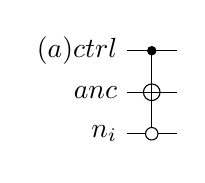
\begin{tikzpicture}[scale=1.000000,x=1pt,y=1pt]
\filldraw[color=white] (0.000000, -7.500000) rectangle (18.000000, 37.500000);
% Drawing wires
% Line 1: ctrl W \text{(a) }ctrl
\draw[color=black] (0.000000,30.000000) -- (18.000000,30.000000);
\draw[color=black] (0.000000,30.000000) node[left] {$\text{(a) }ctrl$};
% Line 2: anc W anc
\draw[color=black] (0.000000,15.000000) -- (18.000000,15.000000);
\draw[color=black] (0.000000,15.000000) node[left] {$anc$};
% Line 3: i W n_i
\draw[color=black] (0.000000,0.000000) -- (18.000000,0.000000);
\draw[color=black] (0.000000,0.000000) node[left] {$n_i$};
% Done with wires; drawing gates
% Line 5: -i +anc ctrl
\draw (9.000000,30.000000) -- (9.000000,0.000000);
\draw[fill=white] (9.000000, 0.000000) circle(2.250000pt);
\begin{scope}
\draw[fill=white] (9.000000, 15.000000) circle(3.000000pt);
\clip (9.000000, 15.000000) circle(3.000000pt);
\draw (6.000000, 15.000000) -- (12.000000, 15.000000);
\draw (9.000000, 12.000000) -- (9.000000, 18.000000);
\end{scope}
\filldraw (9.000000, 30.000000) circle(1.500000pt);
% Done with gates; drawing ending labels
% Done with ending labels; drawing cut lines and comments
% Done with comments
\end{tikzpicture}

        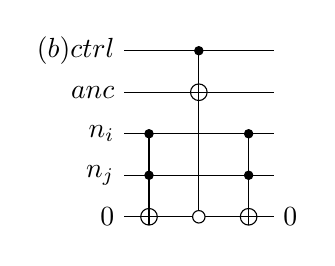
\begin{tikzpicture}[scale=1.000000,x=1pt,y=1pt]
\filldraw[color=white] (0.000000, -7.500000) rectangle (54.000000, 67.500000);
% Drawing wires
% Line 1: ctrl W \text{(b) }ctrl
\draw[color=black] (0.000000,60.000000) -- (54.000000,60.000000);
\draw[color=black] (0.000000,60.000000) node[left] {$\text{(b) }ctrl$};
% Line 2: anc W anc
\draw[color=black] (0.000000,45.000000) -- (54.000000,45.000000);
\draw[color=black] (0.000000,45.000000) node[left] {$anc$};
% Line 3: i W n_i
\draw[color=black] (0.000000,30.000000) -- (54.000000,30.000000);
\draw[color=black] (0.000000,30.000000) node[left] {$n_i$};
% Line 4: j W n_j
\draw[color=black] (0.000000,15.000000) -- (54.000000,15.000000);
\draw[color=black] (0.000000,15.000000) node[left] {$n_j$};
% Line 5: clean0 W 0 0
\draw[color=black] (0.000000,0.000000) -- (54.000000,0.000000);
\draw[color=black] (0.000000,0.000000) node[left] {$0$};
% Done with wires; drawing gates
% Line 7: i j +clean0
\draw (9.000000,30.000000) -- (9.000000,0.000000);
\filldraw (9.000000, 30.000000) circle(1.500000pt);
\filldraw (9.000000, 15.000000) circle(1.500000pt);
\begin{scope}
\draw[fill=white] (9.000000, 0.000000) circle(3.000000pt);
\clip (9.000000, 0.000000) circle(3.000000pt);
\draw (6.000000, 0.000000) -- (12.000000, 0.000000);
\draw (9.000000, -3.000000) -- (9.000000, 3.000000);
\end{scope}
% Line 8: -clean0 ctrl +anc
\draw (27.000000,60.000000) -- (27.000000,0.000000);
\draw[fill=white] (27.000000, 0.000000) circle(2.250000pt);
\filldraw (27.000000, 60.000000) circle(1.500000pt);
\begin{scope}
\draw[fill=white] (27.000000, 45.000000) circle(3.000000pt);
\clip (27.000000, 45.000000) circle(3.000000pt);
\draw (24.000000, 45.000000) -- (30.000000, 45.000000);
\draw (27.000000, 42.000000) -- (27.000000, 48.000000);
\end{scope}
% Line 9: i j +clean0
\draw (45.000000,30.000000) -- (45.000000,0.000000);
\filldraw (45.000000, 30.000000) circle(1.500000pt);
\filldraw (45.000000, 15.000000) circle(1.500000pt);
\begin{scope}
\draw[fill=white] (45.000000, 0.000000) circle(3.000000pt);
\clip (45.000000, 0.000000) circle(3.000000pt);
\draw (42.000000, 0.000000) -- (48.000000, 0.000000);
\draw (45.000000, -3.000000) -- (45.000000, 3.000000);
\end{scope}
% Done with gates; drawing ending labels
\draw[color=black] (54.000000,0.000000) node[right] {$0$};
% Done with ending labels; drawing cut lines and comments
% Done with comments
\end{tikzpicture}

    }
    \mbox{
        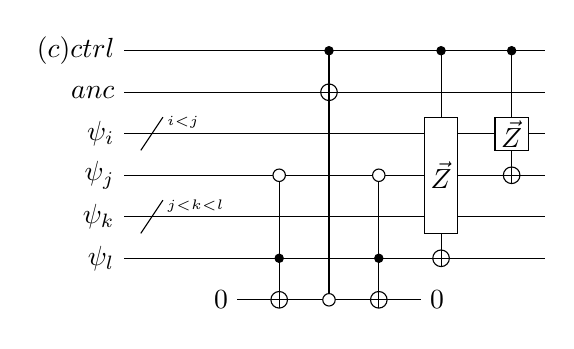
\begin{tikzpicture}[scale=1.000000,x=1pt,y=1pt]
\filldraw[color=white] (0.000000, -7.500000) rectangle (152.000000, 97.500000);
% Drawing wires
% Line 1: ctrl W \text{(c) }ctrl
\draw[color=black] (0.000000,90.000000) -- (152.000000,90.000000);
\draw[color=black] (0.000000,90.000000) node[left] {$\text{(c) }ctrl$};
% Line 2: anc W anc
\draw[color=black] (0.000000,75.000000) -- (152.000000,75.000000);
\draw[color=black] (0.000000,75.000000) node[left] {$anc$};
% Line 3: i W \psi_i
\draw[color=black] (0.000000,60.000000) -- (152.000000,60.000000);
\draw[color=black] (0.000000,60.000000) node[left] {$\psi_i$};
% Line 4: j W \psi_j
\draw[color=black] (0.000000,45.000000) -- (152.000000,45.000000);
\draw[color=black] (0.000000,45.000000) node[left] {$\psi_j$};
% Line 5: k W \psi_k
\draw[color=black] (0.000000,30.000000) -- (152.000000,30.000000);
\draw[color=black] (0.000000,30.000000) node[left] {$\psi_k$};
% Line 6: l W \psi_l
\draw[color=black] (0.000000,15.000000) -- (152.000000,15.000000);
\draw[color=black] (0.000000,15.000000) node[left] {$\psi_l$};
% Line 7: clean0 W 0 0
\draw[color=black] (33.500000,0.000000) -- (114.500000,0.000000);
% Done with wires; drawing gates
% Line 9: i / ^{i<j}
\draw (6.000000, 54.000000) -- (14.000000, 66.000000);
\draw (12.000000, 63.000000) node[right] {$\scriptstyle{^{i<j}}$};
% Line 10: k / ^{j<k<l}
\draw (6.000000, 24.000000) -- (14.000000, 36.000000);
\draw (12.000000, 33.000000) node[right] {$\scriptstyle{^{j<k<l}}$};
% Line 11: ctrl anc i j k l LABEL
% Line 13: clean0 START
\draw[color=black] (41.000000,0.000000) node[fill=white,left,minimum height=15.000000pt,minimum width=15.000000pt,inner sep=0pt] {\phantom{$0$}};
\draw[color=black] (41.000000,0.000000) node[left] {$0$};
% Line 14: -j l +clean0
\draw (56.000000,45.000000) -- (56.000000,0.000000);
\draw[fill=white] (56.000000, 45.000000) circle(2.250000pt);
\filldraw (56.000000, 15.000000) circle(1.500000pt);
\begin{scope}
\draw[fill=white] (56.000000, 0.000000) circle(3.000000pt);
\clip (56.000000, 0.000000) circle(3.000000pt);
\draw (53.000000, 0.000000) -- (59.000000, 0.000000);
\draw (56.000000, -3.000000) -- (56.000000, 3.000000);
\end{scope}
% Line 15: ctrl +anc -clean0
\draw (74.000000,90.000000) -- (74.000000,0.000000);
\filldraw (74.000000, 90.000000) circle(1.500000pt);
\begin{scope}
\draw[fill=white] (74.000000, 75.000000) circle(3.000000pt);
\clip (74.000000, 75.000000) circle(3.000000pt);
\draw (71.000000, 75.000000) -- (77.000000, 75.000000);
\draw (74.000000, 72.000000) -- (74.000000, 78.000000);
\end{scope}
\draw[fill=white] (74.000000, 0.000000) circle(2.250000pt);
% Line 16: -j l +clean0
\draw (92.000000,45.000000) -- (92.000000,0.000000);
\draw[fill=white] (92.000000, 45.000000) circle(2.250000pt);
\filldraw (92.000000, 15.000000) circle(1.500000pt);
\begin{scope}
\draw[fill=white] (92.000000, 0.000000) circle(3.000000pt);
\clip (92.000000, 0.000000) circle(3.000000pt);
\draw (89.000000, 0.000000) -- (95.000000, 0.000000);
\draw (92.000000, -3.000000) -- (92.000000, 3.000000);
\end{scope}
% Line 17: clean0 END
\draw[color=black] (107.000000,0.000000) node[fill=white,right,minimum height=15.000000pt,minimum width=15.000000pt,inner sep=0pt] {\phantom{$0$}};
\draw[color=black] (107.000000,0.000000) node[right] {$0$};
% Line 19: i j k G $\vec{Z}$ +l ctrl
\draw (114.500000,90.000000) -- (114.500000,15.000000);
\begin{scope}
\draw[fill=white] (114.500000, 45.000000) +(-45.000000:8.485281pt and 29.698485pt) -- +(45.000000:8.485281pt and 29.698485pt) -- +(135.000000:8.485281pt and 29.698485pt) -- +(225.000000:8.485281pt and 29.698485pt) -- cycle;
\clip (114.500000, 45.000000) +(-45.000000:8.485281pt and 29.698485pt) -- +(45.000000:8.485281pt and 29.698485pt) -- +(135.000000:8.485281pt and 29.698485pt) -- +(225.000000:8.485281pt and 29.698485pt) -- cycle;
\draw (114.500000, 45.000000) node {$\vec{Z}$};
\end{scope}
\begin{scope}
\draw[fill=white] (114.500000, 15.000000) circle(3.000000pt);
\clip (114.500000, 15.000000) circle(3.000000pt);
\draw (111.500000, 15.000000) -- (117.500000, 15.000000);
\draw (114.500000, 12.000000) -- (114.500000, 18.000000);
\end{scope}
\filldraw (114.500000, 90.000000) circle(1.500000pt);
% Line 20: i G $\vec{Z}$ +j ctrl
\draw (140.000000,90.000000) -- (140.000000,45.000000);
\begin{scope}
\draw[fill=white] (140.000000, 60.000000) +(-45.000000:8.485281pt and 8.485281pt) -- +(45.000000:8.485281pt and 8.485281pt) -- +(135.000000:8.485281pt and 8.485281pt) -- +(225.000000:8.485281pt and 8.485281pt) -- cycle;
\clip (140.000000, 60.000000) +(-45.000000:8.485281pt and 8.485281pt) -- +(45.000000:8.485281pt and 8.485281pt) -- +(135.000000:8.485281pt and 8.485281pt) -- +(225.000000:8.485281pt and 8.485281pt) -- cycle;
\draw (140.000000, 60.000000) node {$\vec{Z}$};
\end{scope}
\begin{scope}
\draw[fill=white] (140.000000, 45.000000) circle(3.000000pt);
\clip (140.000000, 45.000000) circle(3.000000pt);
\draw (137.000000, 45.000000) -- (143.000000, 45.000000);
\draw (140.000000, 42.000000) -- (140.000000, 48.000000);
\end{scope}
\filldraw (140.000000, 90.000000) circle(1.500000pt);
% Done with gates; drawing ending labels
% Done with ending labels; drawing cut lines and comments
% Done with comments
\end{tikzpicture}

        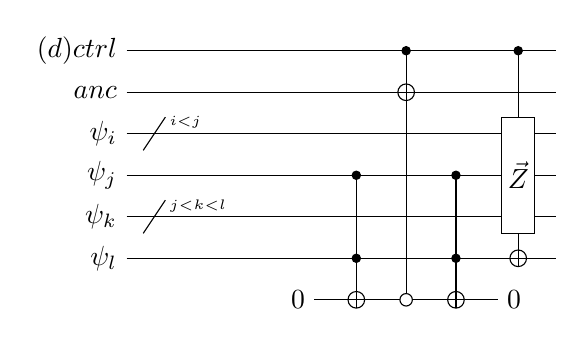
\begin{tikzpicture}[scale=1.000000,x=1pt,y=1pt]
\filldraw[color=white] (0.000000, -7.500000) rectangle (155.000000, 97.500000);
% Drawing wires
% Line 1: ctrl W \text{(d) }ctrl
\draw[color=black] (0.000000,90.000000) -- (155.000000,90.000000);
\draw[color=black] (0.000000,90.000000) node[left] {$\text{(d) }ctrl$};
% Line 2: anc W anc
\draw[color=black] (0.000000,75.000000) -- (155.000000,75.000000);
\draw[color=black] (0.000000,75.000000) node[left] {$anc$};
% Line 3: i W \psi_i
\draw[color=black] (0.000000,60.000000) -- (155.000000,60.000000);
\draw[color=black] (0.000000,60.000000) node[left] {$\psi_i$};
% Line 4: j W \psi_j
\draw[color=black] (0.000000,45.000000) -- (155.000000,45.000000);
\draw[color=black] (0.000000,45.000000) node[left] {$\psi_j$};
% Line 5: k W \psi_k
\draw[color=black] (0.000000,30.000000) -- (155.000000,30.000000);
\draw[color=black] (0.000000,30.000000) node[left] {$\psi_k$};
% Line 6: l W \psi_l
\draw[color=black] (0.000000,15.000000) -- (155.000000,15.000000);
\draw[color=black] (0.000000,15.000000) node[left] {$\psi_l$};
% Line 7: clean0 W 0 0
\draw[color=black] (60.500000,0.000000) -- (141.500000,0.000000);
% Done with wires; drawing gates
% Line 9: i / ^{i<j}
\draw (6.000000, 54.000000) -- (14.000000, 66.000000);
\draw (12.000000, 63.000000) node[right] {$\scriptstyle{^{i<j}}$};
% Line 10: k / ^{j<k<l}
\draw (6.000000, 24.000000) -- (14.000000, 36.000000);
\draw (12.000000, 33.000000) node[right] {$\scriptstyle{^{j<k<l}}$};
% Line 11: ctrl anc i j k l clean0 LABEL
% Line 13: clean0 START
\draw[color=black] (68.000000,0.000000) node[fill=white,left,minimum height=15.000000pt,minimum width=15.000000pt,inner sep=0pt] {\phantom{$0$}};
\draw[color=black] (68.000000,0.000000) node[left] {$0$};
% Line 14: j l +clean0
\draw (83.000000,45.000000) -- (83.000000,0.000000);
\filldraw (83.000000, 45.000000) circle(1.500000pt);
\filldraw (83.000000, 15.000000) circle(1.500000pt);
\begin{scope}
\draw[fill=white] (83.000000, 0.000000) circle(3.000000pt);
\clip (83.000000, 0.000000) circle(3.000000pt);
\draw (80.000000, 0.000000) -- (86.000000, 0.000000);
\draw (83.000000, -3.000000) -- (83.000000, 3.000000);
\end{scope}
% Line 15: ctrl +anc -clean0
\draw (101.000000,90.000000) -- (101.000000,0.000000);
\filldraw (101.000000, 90.000000) circle(1.500000pt);
\begin{scope}
\draw[fill=white] (101.000000, 75.000000) circle(3.000000pt);
\clip (101.000000, 75.000000) circle(3.000000pt);
\draw (98.000000, 75.000000) -- (104.000000, 75.000000);
\draw (101.000000, 72.000000) -- (101.000000, 78.000000);
\end{scope}
\draw[fill=white] (101.000000, 0.000000) circle(2.250000pt);
% Line 16: j l +clean0
\draw (119.000000,45.000000) -- (119.000000,0.000000);
\filldraw (119.000000, 45.000000) circle(1.500000pt);
\filldraw (119.000000, 15.000000) circle(1.500000pt);
\begin{scope}
\draw[fill=white] (119.000000, 0.000000) circle(3.000000pt);
\clip (119.000000, 0.000000) circle(3.000000pt);
\draw (116.000000, 0.000000) -- (122.000000, 0.000000);
\draw (119.000000, -3.000000) -- (119.000000, 3.000000);
\end{scope}
% Line 17: clean0 END
\draw[color=black] (134.000000,0.000000) node[fill=white,right,minimum height=15.000000pt,minimum width=15.000000pt,inner sep=0pt] {\phantom{$0$}};
\draw[color=black] (134.000000,0.000000) node[right] {$0$};
% Line 19: i j k G $\vec{Z}$ +l ctrl
\draw (141.500000,90.000000) -- (141.500000,15.000000);
\begin{scope}
\draw[fill=white] (141.500000, 45.000000) +(-45.000000:8.485281pt and 29.698485pt) -- +(45.000000:8.485281pt and 29.698485pt) -- +(135.000000:8.485281pt and 29.698485pt) -- +(225.000000:8.485281pt and 29.698485pt) -- cycle;
\clip (141.500000, 45.000000) +(-45.000000:8.485281pt and 29.698485pt) -- +(45.000000:8.485281pt and 29.698485pt) -- +(135.000000:8.485281pt and 29.698485pt) -- +(225.000000:8.485281pt and 29.698485pt) -- cycle;
\draw (141.500000, 45.000000) node {$\vec{Z}$};
\end{scope}
\begin{scope}
\draw[fill=white] (141.500000, 15.000000) circle(3.000000pt);
\clip (141.500000, 15.000000) circle(3.000000pt);
\draw (138.500000, 15.000000) -- (144.500000, 15.000000);
\draw (141.500000, 12.000000) -- (141.500000, 18.000000);
\end{scope}
\filldraw (141.500000, 90.000000) circle(1.500000pt);
% Done with gates; drawing ending labels
% Done with ending labels; drawing cut lines and comments
% Done with comments
\end{tikzpicture}

    }
    \caption{
        \textbf{Block-Encoding Products of Fermionic Ladder Operators}
        In subfigure a, a block-encoding for the fermionic number operator acting on the $j^\text{th}$ mode is given.
        In subfigure b, a block-encoding for the product of two fermionic number operators acting on the $j^\text{th}$ and $l^\text{th}$ modes is given.
        In subfigure c, a block-encoding for the operator $b_j^\dagger b_l$ with $i \neq l$ is given.
        In subfigure d, a block-encoding for the operator $b_j^\dagger b_j b_l$ with $i \neq l$ is given.
    }
    \label{fig:fermionic-products-be}
\end{figure}

As a simple example where we can produce a more efficient construction, consider the fermionic number operator: $b_j^\dagger b_j$.
Note the behavior of the conjoined operator on an arbitrary quantum state:
\begin{equation}
    \begin{split}
        b_j^\dagger b_j \ket{\psi_{b_j}} = \begin{cases} 
            \ket{1} & \text{when $\ket{\psi_{b_j}}$ is $\ket{1}$} \\
            0 & \text{when $\ket{\psi_{b_j}}$ is $\ket{0}$} \\
                                        \end{cases}
    \end{split}
\end{equation}
If the $j^\text{th}$ mode is unoccupied, the state will be zeroed-out.
If the $j^\text{th}$ mode is occupied, then the state is left unchanged.
We can describe this action using the circuit shown in subfigure \ref{fig:fermionic-products-be}a.
The Toffoli gate flips the block-encoding ancilla outside the subspace if the control is on and the $j^\text{th}$ mode is unoccupied.
Otherwise, the state of the system and the block-encoding ancilla are left unchanged.
Block-encoding this operator as the product of the block-encodings for $b_j^\dagger$ and $b_j$ would require $2$ Toffoli gates and $2$ block-encoding ancillae.
The construction given here requires only one Toffoli gate and one block-encoding ancilla.

For a more general product of two fermionic ladder operators, a block-encoding circuit for the operator $b_j^\dagger b_l$ is given in subfigure \ref{fig:fermionic-products-be}c.
For this operator, we can infer that the state will be zeroed-out \textit{unless} both the $j^\text{th}$ mode is unoccupied and the $l^\text{th}$ mode is occupied.
The temporary logical-AND of these two conditions is stored in a clean ancilla.
If the control qubit is on and these two conditions on the system are not true, then the block-encoding ancilla is flipped outside of the encoded subspace.
After the state of the block-encoding ancilla is determined, the system is updated by applying the two operators onto the system in order: $b_l$ then $b_j^\dagger$.
These operators are applied using similar operators of the form $\vec{Z}X$ which applies the appropriate sign flip based on the occupation of the preceeding modes and updates the occupation of the fermionic mode.
This block-encoding circuit has an optimal rescaling factor ($\lambda = 1$), requires one block-encoding ancilla, and uses two Toffoli gates.


This construction can be generalized to an arbitrary product of ladder operators.
Let $B$ represent the number of active modes in a term where we define an active mode as a mode that has a ladder operator applied to it.
For example, the term $b_i b_j^\dagger b_k b_l^\dagger b_l$ has $4$ active modes.
Each active mode will contribute a new control on the state of the mode.
For a general product of fermionic ladder operators, a block-encoding circuit of this form will have an optimal rescaling factor ($\lambda = 1$), require only one block-encoding ancilla, and use $B$ Toffoli gates.
The count of $B$ Toffoli gates assumes that each $B$-controlled NOT gate is decomposed into a series of $B-1$ Toffoli gates as described in Appendix \ref{sec:elbows}.

\ws{
A natural question to ask is how do these constructions compare with using an LCU block-encoding after applying the Jordan-Wigner transformation \cite{}?
The Jordan-Wigner transformation maps each fermionic ladder operator (or number operator) to a sum of two Pauli operators.
For an arbitrary product of fermionic ladder operators, expanding these linear combinations results in $2^{B}$ Paulis.
The number of non-Clifford gates for LCU scales linearly with the number of operators and hence would scale exponentially with $B$ under this construction.
Alternatively, one could construct LCU block-encodings for each of the ladder operators in a term by applying the Jordan-Wigner transformation to each ladder operator (or number operator) independently.
The product of these block-encodings would then give a block-encoding of the term.
For each ladder operator (or number operator), an LCU block-encoding would require one Toffoli gate and one ancilla qubit.
A block-encoding of the whole term using this construction would then require $B$ Toffoli gates and $B$ block-encoding ancillae.
}

\subsection{Linear Combinations of Fermionic Ladder Operators}


As discussed in subsection \ref{subsec:be-products}, a block-encoding for a linear combination of operators can be constructed using the LCO framework (Theorem \ref{th:lco}).
In this subsection, we show how to construct block-encodings of linear combinations of products of fermionic ladder operators that use fewer quantum resources than are required by an LCO construction.
In particular, we give a generalizable construction for a product of fermionic ladder operators plus its hermitian conjugate.
However, we note that the strategies we present here are not restricted only to these linear combinations.

\begin{figure}
    \mbox{
        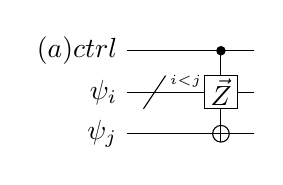
\begin{tikzpicture}[scale=1.000000,x=1pt,y=1pt]
\filldraw[color=white] (0.000000, -7.500000) rectangle (46.000000, 37.500000);
% Drawing wires
% Line 1: a W \text{(a) }ctrl
\draw[color=black] (0.000000,30.000000) -- (46.000000,30.000000);
\draw[color=black] (0.000000,30.000000) node[left] {$\text{(a) }ctrl$};
% Line 2: b W \psi_i
\draw[color=black] (0.000000,15.000000) -- (46.000000,15.000000);
\draw[color=black] (0.000000,15.000000) node[left] {$\psi_i$};
% Line 3: c W \psi_j
\draw[color=black] (0.000000,0.000000) -- (46.000000,0.000000);
\draw[color=black] (0.000000,0.000000) node[left] {$\psi_j$};
% Done with wires; drawing gates
% Line 5: b / ^{i<j}
\draw (6.000000, 9.000000) -- (14.000000, 21.000000);
\draw (12.000000, 18.000000) node[right] {$\scriptstyle{^{i<j}}$};
% Line 6: a b c LABEL width=-10
% Line 7: b G $\vec{Z}$ a +c
\draw (34.000000,30.000000) -- (34.000000,0.000000);
\begin{scope}
\draw[fill=white] (34.000000, 15.000000) +(-45.000000:8.485281pt and 8.485281pt) -- +(45.000000:8.485281pt and 8.485281pt) -- +(135.000000:8.485281pt and 8.485281pt) -- +(225.000000:8.485281pt and 8.485281pt) -- cycle;
\clip (34.000000, 15.000000) +(-45.000000:8.485281pt and 8.485281pt) -- +(45.000000:8.485281pt and 8.485281pt) -- +(135.000000:8.485281pt and 8.485281pt) -- +(225.000000:8.485281pt and 8.485281pt) -- cycle;
\draw (34.000000, 15.000000) node {$\vec{Z}$};
\end{scope}
\filldraw (34.000000, 30.000000) circle(1.500000pt);
\begin{scope}
\draw[fill=white] (34.000000, 0.000000) circle(3.000000pt);
\clip (34.000000, 0.000000) circle(3.000000pt);
\draw (31.000000, 0.000000) -- (37.000000, 0.000000);
\draw (34.000000, -3.000000) -- (34.000000, 3.000000);
\end{scope}
% Done with gates; drawing ending labels
% Done with ending labels; drawing cut lines and comments
% Done with comments
\end{tikzpicture}

        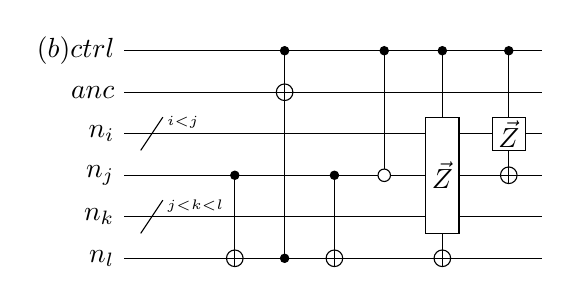
\begin{tikzpicture}[scale=1.000000,x=1pt,y=1pt]
\filldraw[color=white] (0.000000, -7.500000) rectangle (151.000000, 82.500000);
% Drawing wires
% Line 1: c W \text{(b) }ctrl
\draw[color=black] (0.000000,75.000000) -- (151.000000,75.000000);
\draw[color=black] (0.000000,75.000000) node[left] {$\text{(b) }ctrl$};
% Line 2: a W anc
\draw[color=black] (0.000000,60.000000) -- (151.000000,60.000000);
\draw[color=black] (0.000000,60.000000) node[left] {$anc$};
% Line 3: i W n_i
\draw[color=black] (0.000000,45.000000) -- (151.000000,45.000000);
\draw[color=black] (0.000000,45.000000) node[left] {$n_i$};
% Line 4: j W n_j
\draw[color=black] (0.000000,30.000000) -- (151.000000,30.000000);
\draw[color=black] (0.000000,30.000000) node[left] {$n_j$};
% Line 5: k W n_k
\draw[color=black] (0.000000,15.000000) -- (151.000000,15.000000);
\draw[color=black] (0.000000,15.000000) node[left] {$n_k$};
% Line 6: l W n_l
\draw[color=black] (0.000000,0.000000) -- (151.000000,0.000000);
\draw[color=black] (0.000000,0.000000) node[left] {$n_l$};
% Done with wires; drawing gates
% Line 8: i / ^{i<j}
\draw (6.000000, 39.000000) -- (14.000000, 51.000000);
\draw (12.000000, 48.000000) node[right] {$\scriptstyle{^{i<j}}$};
% Line 9: k / ^{j<k<l}
\draw (6.000000, 9.000000) -- (14.000000, 21.000000);
\draw (12.000000, 18.000000) node[right] {$\scriptstyle{^{j<k<l}}$};
% Line 10: c a i j k l LABEL width=-1
% Line 11: j +l
\draw (40.000000,30.000000) -- (40.000000,0.000000);
\filldraw (40.000000, 30.000000) circle(1.500000pt);
\begin{scope}
\draw[fill=white] (40.000000, 0.000000) circle(3.000000pt);
\clip (40.000000, 0.000000) circle(3.000000pt);
\draw (37.000000, 0.000000) -- (43.000000, 0.000000);
\draw (40.000000, -3.000000) -- (40.000000, 3.000000);
\end{scope}
% Line 12: c l +a
\draw (58.000000,75.000000) -- (58.000000,0.000000);
\filldraw (58.000000, 75.000000) circle(1.500000pt);
\filldraw (58.000000, 0.000000) circle(1.500000pt);
\begin{scope}
\draw[fill=white] (58.000000, 60.000000) circle(3.000000pt);
\clip (58.000000, 60.000000) circle(3.000000pt);
\draw (55.000000, 60.000000) -- (61.000000, 60.000000);
\draw (58.000000, 57.000000) -- (58.000000, 63.000000);
\end{scope}
% Line 13: j +l
\draw (76.000000,30.000000) -- (76.000000,0.000000);
\filldraw (76.000000, 30.000000) circle(1.500000pt);
\begin{scope}
\draw[fill=white] (76.000000, 0.000000) circle(3.000000pt);
\clip (76.000000, 0.000000) circle(3.000000pt);
\draw (73.000000, 0.000000) -- (79.000000, 0.000000);
\draw (76.000000, -3.000000) -- (76.000000, 3.000000);
\end{scope}
% Line 14: c -j
\draw (94.000000,75.000000) -- (94.000000,30.000000);
\filldraw (94.000000, 75.000000) circle(1.500000pt);
\draw[fill=white] (94.000000, 30.000000) circle(2.250000pt);
% Line 16: i j k G $\vec{Z}$ c +l
\draw (115.000000,75.000000) -- (115.000000,0.000000);
\begin{scope}
\draw[fill=white] (115.000000, 30.000000) +(-45.000000:8.485281pt and 29.698485pt) -- +(45.000000:8.485281pt and 29.698485pt) -- +(135.000000:8.485281pt and 29.698485pt) -- +(225.000000:8.485281pt and 29.698485pt) -- cycle;
\clip (115.000000, 30.000000) +(-45.000000:8.485281pt and 29.698485pt) -- +(45.000000:8.485281pt and 29.698485pt) -- +(135.000000:8.485281pt and 29.698485pt) -- +(225.000000:8.485281pt and 29.698485pt) -- cycle;
\draw (115.000000, 30.000000) node {$\vec{Z}$};
\end{scope}
\filldraw (115.000000, 75.000000) circle(1.500000pt);
\begin{scope}
\draw[fill=white] (115.000000, 0.000000) circle(3.000000pt);
\clip (115.000000, 0.000000) circle(3.000000pt);
\draw (112.000000, 0.000000) -- (118.000000, 0.000000);
\draw (115.000000, -3.000000) -- (115.000000, 3.000000);
\end{scope}
% Line 17: i G $\vec{Z}$ c +j
\draw (139.000000,75.000000) -- (139.000000,30.000000);
\begin{scope}
\draw[fill=white] (139.000000, 45.000000) +(-45.000000:8.485281pt and 8.485281pt) -- +(45.000000:8.485281pt and 8.485281pt) -- +(135.000000:8.485281pt and 8.485281pt) -- +(225.000000:8.485281pt and 8.485281pt) -- cycle;
\clip (139.000000, 45.000000) +(-45.000000:8.485281pt and 8.485281pt) -- +(45.000000:8.485281pt and 8.485281pt) -- +(135.000000:8.485281pt and 8.485281pt) -- +(225.000000:8.485281pt and 8.485281pt) -- cycle;
\draw (139.000000, 45.000000) node {$\vec{Z}$};
\end{scope}
\filldraw (139.000000, 75.000000) circle(1.500000pt);
\begin{scope}
\draw[fill=white] (139.000000, 30.000000) circle(3.000000pt);
\clip (139.000000, 30.000000) circle(3.000000pt);
\draw (136.000000, 30.000000) -- (142.000000, 30.000000);
\draw (139.000000, 27.000000) -- (139.000000, 33.000000);
\end{scope}
% Done with gates; drawing ending labels
% Done with ending labels; drawing cut lines and comments
% Done with comments
\end{tikzpicture}

    }
    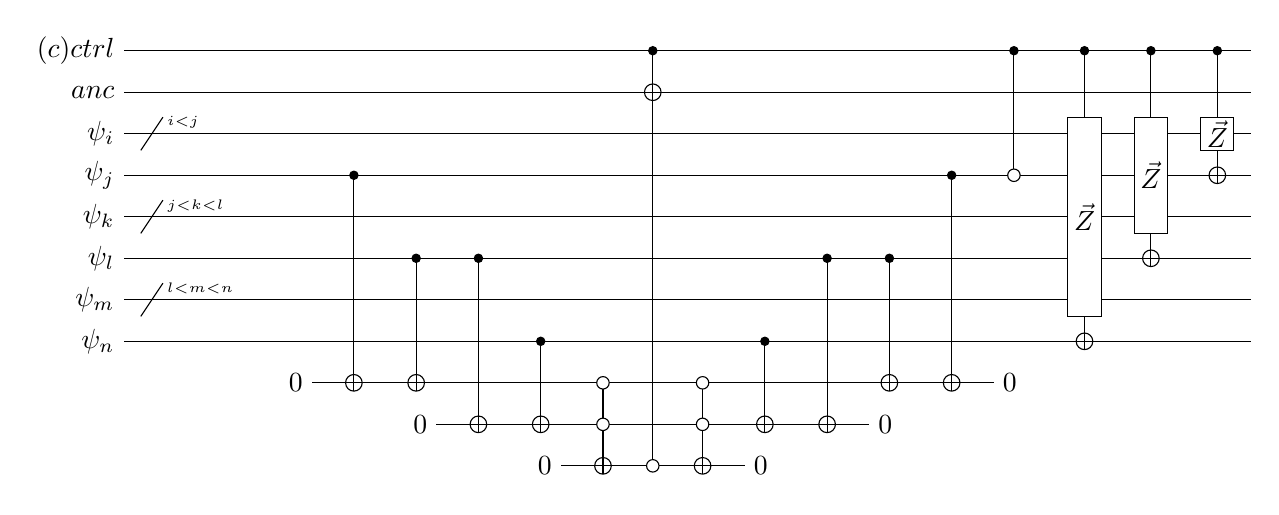
\begin{tikzpicture}[scale=1.000000,x=1pt,y=1pt]
\filldraw[color=white] (0.000000, -7.500000) rectangle (407.000000, 157.500000);
% Drawing wires
% Line 1: ctrl W \text{(c) }ctrl
\draw[color=black] (0.000000,150.000000) -- (407.000000,150.000000);
\draw[color=black] (0.000000,150.000000) node[left] {$\text{(c) }ctrl$};
% Line 2: anc W anc
\draw[color=black] (0.000000,135.000000) -- (407.000000,135.000000);
\draw[color=black] (0.000000,135.000000) node[left] {$anc$};
% Line 3: i W \psi_i
\draw[color=black] (0.000000,120.000000) -- (407.000000,120.000000);
\draw[color=black] (0.000000,120.000000) node[left] {$\psi_i$};
% Line 4: j W \psi_j
\draw[color=black] (0.000000,105.000000) -- (407.000000,105.000000);
\draw[color=black] (0.000000,105.000000) node[left] {$\psi_j$};
% Line 5: k W \psi_k
\draw[color=black] (0.000000,90.000000) -- (407.000000,90.000000);
\draw[color=black] (0.000000,90.000000) node[left] {$\psi_k$};
% Line 6: l W \psi_l
\draw[color=black] (0.000000,75.000000) -- (407.000000,75.000000);
\draw[color=black] (0.000000,75.000000) node[left] {$\psi_l$};
% Line 7: m W \psi_m
\draw[color=black] (0.000000,60.000000) -- (407.000000,60.000000);
\draw[color=black] (0.000000,60.000000) node[left] {$\psi_m$};
% Line 8: n W \psi_n
\draw[color=black] (0.000000,45.000000) -- (407.000000,45.000000);
\draw[color=black] (0.000000,45.000000) node[left] {$\psi_n$};
% Line 9: clean0 W 0 0
\draw[color=black] (60.500000,30.000000) -- (321.500000,30.000000);
% Line 10: clean1 W 0 0
\draw[color=black] (105.500000,15.000000) -- (276.500000,15.000000);
% Line 11: clean2 W 0 0
\draw[color=black] (150.500000,0.000000) -- (231.500000,0.000000);
% Done with wires; drawing gates
% Line 13: i / ^{i<j}
\draw (6.000000, 114.000000) -- (14.000000, 126.000000);
\draw (12.000000, 123.000000) node[right] {$\scriptstyle{^{i<j}}$};
% Line 14: k / ^{j<k<l}
\draw (6.000000, 84.000000) -- (14.000000, 96.000000);
\draw (12.000000, 93.000000) node[right] {$\scriptstyle{^{j<k<l}}$};
% Line 15: m / ^{l<m<n}
\draw (6.000000, 54.000000) -- (14.000000, 66.000000);
\draw (12.000000, 63.000000) node[right] {$\scriptstyle{^{l<m<n}}$};
% Line 16: ctrl anc i j k l m n clean0 LABEL
% Line 17: clean0 START
\draw[color=black] (68.000000,30.000000) node[fill=white,left,minimum height=15.000000pt,minimum width=15.000000pt,inner sep=0pt] {\phantom{$0$}};
\draw[color=black] (68.000000,30.000000) node[left] {$0$};
% Line 18: j +clean0
\draw (83.000000,105.000000) -- (83.000000,30.000000);
\filldraw (83.000000, 105.000000) circle(1.500000pt);
\begin{scope}
\draw[fill=white] (83.000000, 30.000000) circle(3.000000pt);
\clip (83.000000, 30.000000) circle(3.000000pt);
\draw (80.000000, 30.000000) -- (86.000000, 30.000000);
\draw (83.000000, 27.000000) -- (83.000000, 33.000000);
\end{scope}
% Line 19: l +clean0
\draw (105.500000,75.000000) -- (105.500000,30.000000);
\filldraw (105.500000, 75.000000) circle(1.500000pt);
\begin{scope}
\draw[fill=white] (105.500000, 30.000000) circle(3.000000pt);
\clip (105.500000, 30.000000) circle(3.000000pt);
\draw (102.500000, 30.000000) -- (108.500000, 30.000000);
\draw (105.500000, 27.000000) -- (105.500000, 33.000000);
\end{scope}
% Line 20: clean1 START
\draw[color=black] (113.000000,15.000000) node[fill=white,left,minimum height=15.000000pt,minimum width=15.000000pt,inner sep=0pt] {\phantom{$0$}};
\draw[color=black] (113.000000,15.000000) node[left] {$0$};
% Line 21: l +clean1
\draw (128.000000,75.000000) -- (128.000000,15.000000);
\filldraw (128.000000, 75.000000) circle(1.500000pt);
\begin{scope}
\draw[fill=white] (128.000000, 15.000000) circle(3.000000pt);
\clip (128.000000, 15.000000) circle(3.000000pt);
\draw (125.000000, 15.000000) -- (131.000000, 15.000000);
\draw (128.000000, 12.000000) -- (128.000000, 18.000000);
\end{scope}
% Line 22: n +clean1
\draw (150.500000,45.000000) -- (150.500000,15.000000);
\filldraw (150.500000, 45.000000) circle(1.500000pt);
\begin{scope}
\draw[fill=white] (150.500000, 15.000000) circle(3.000000pt);
\clip (150.500000, 15.000000) circle(3.000000pt);
\draw (147.500000, 15.000000) -- (153.500000, 15.000000);
\draw (150.500000, 12.000000) -- (150.500000, 18.000000);
\end{scope}
% Line 23: clean2 START
\draw[color=black] (158.000000,0.000000) node[fill=white,left,minimum height=15.000000pt,minimum width=15.000000pt,inner sep=0pt] {\phantom{$0$}};
\draw[color=black] (158.000000,0.000000) node[left] {$0$};
% Line 24: -clean0 -clean1 +clean2
\draw (173.000000,30.000000) -- (173.000000,0.000000);
\draw[fill=white] (173.000000, 30.000000) circle(2.250000pt);
\draw[fill=white] (173.000000, 15.000000) circle(2.250000pt);
\begin{scope}
\draw[fill=white] (173.000000, 0.000000) circle(3.000000pt);
\clip (173.000000, 0.000000) circle(3.000000pt);
\draw (170.000000, 0.000000) -- (176.000000, 0.000000);
\draw (173.000000, -3.000000) -- (173.000000, 3.000000);
\end{scope}
% Line 25: ctrl -clean2 +anc
\draw (191.000000,150.000000) -- (191.000000,0.000000);
\filldraw (191.000000, 150.000000) circle(1.500000pt);
\draw[fill=white] (191.000000, 0.000000) circle(2.250000pt);
\begin{scope}
\draw[fill=white] (191.000000, 135.000000) circle(3.000000pt);
\clip (191.000000, 135.000000) circle(3.000000pt);
\draw (188.000000, 135.000000) -- (194.000000, 135.000000);
\draw (191.000000, 132.000000) -- (191.000000, 138.000000);
\end{scope}
% Line 26: -clean0 -clean1 +clean2
\draw (209.000000,30.000000) -- (209.000000,0.000000);
\draw[fill=white] (209.000000, 30.000000) circle(2.250000pt);
\draw[fill=white] (209.000000, 15.000000) circle(2.250000pt);
\begin{scope}
\draw[fill=white] (209.000000, 0.000000) circle(3.000000pt);
\clip (209.000000, 0.000000) circle(3.000000pt);
\draw (206.000000, 0.000000) -- (212.000000, 0.000000);
\draw (209.000000, -3.000000) -- (209.000000, 3.000000);
\end{scope}
% Line 27: clean2 END
\draw[color=black] (224.000000,0.000000) node[fill=white,right,minimum height=15.000000pt,minimum width=15.000000pt,inner sep=0pt] {\phantom{$0$}};
\draw[color=black] (224.000000,0.000000) node[right] {$0$};
% Line 28: n +clean1
\draw (231.500000,45.000000) -- (231.500000,15.000000);
\filldraw (231.500000, 45.000000) circle(1.500000pt);
\begin{scope}
\draw[fill=white] (231.500000, 15.000000) circle(3.000000pt);
\clip (231.500000, 15.000000) circle(3.000000pt);
\draw (228.500000, 15.000000) -- (234.500000, 15.000000);
\draw (231.500000, 12.000000) -- (231.500000, 18.000000);
\end{scope}
% Line 29: l +clean1
\draw (254.000000,75.000000) -- (254.000000,15.000000);
\filldraw (254.000000, 75.000000) circle(1.500000pt);
\begin{scope}
\draw[fill=white] (254.000000, 15.000000) circle(3.000000pt);
\clip (254.000000, 15.000000) circle(3.000000pt);
\draw (251.000000, 15.000000) -- (257.000000, 15.000000);
\draw (254.000000, 12.000000) -- (254.000000, 18.000000);
\end{scope}
% Line 30: clean1 END
\draw[color=black] (269.000000,15.000000) node[fill=white,right,minimum height=15.000000pt,minimum width=15.000000pt,inner sep=0pt] {\phantom{$0$}};
\draw[color=black] (269.000000,15.000000) node[right] {$0$};
% Line 31: l +clean0
\draw (276.500000,75.000000) -- (276.500000,30.000000);
\filldraw (276.500000, 75.000000) circle(1.500000pt);
\begin{scope}
\draw[fill=white] (276.500000, 30.000000) circle(3.000000pt);
\clip (276.500000, 30.000000) circle(3.000000pt);
\draw (273.500000, 30.000000) -- (279.500000, 30.000000);
\draw (276.500000, 27.000000) -- (276.500000, 33.000000);
\end{scope}
% Line 32: j +clean0
\draw (299.000000,105.000000) -- (299.000000,30.000000);
\filldraw (299.000000, 105.000000) circle(1.500000pt);
\begin{scope}
\draw[fill=white] (299.000000, 30.000000) circle(3.000000pt);
\clip (299.000000, 30.000000) circle(3.000000pt);
\draw (296.000000, 30.000000) -- (302.000000, 30.000000);
\draw (299.000000, 27.000000) -- (299.000000, 33.000000);
\end{scope}
% Line 33: clean0 END
\draw[color=black] (314.000000,30.000000) node[fill=white,right,minimum height=15.000000pt,minimum width=15.000000pt,inner sep=0pt] {\phantom{$0$}};
\draw[color=black] (314.000000,30.000000) node[right] {$0$};
% Line 35: ctrl -j
\draw (321.500000,150.000000) -- (321.500000,105.000000);
\filldraw (321.500000, 150.000000) circle(1.500000pt);
\draw[fill=white] (321.500000, 105.000000) circle(2.250000pt);
% Line 37: i j k l m G $\vec{Z}$ ctrl +n
\draw (347.000000,150.000000) -- (347.000000,45.000000);
\begin{scope}
\draw[fill=white] (347.000000, 90.000000) +(-45.000000:8.485281pt and 50.911688pt) -- +(45.000000:8.485281pt and 50.911688pt) -- +(135.000000:8.485281pt and 50.911688pt) -- +(225.000000:8.485281pt and 50.911688pt) -- cycle;
\clip (347.000000, 90.000000) +(-45.000000:8.485281pt and 50.911688pt) -- +(45.000000:8.485281pt and 50.911688pt) -- +(135.000000:8.485281pt and 50.911688pt) -- +(225.000000:8.485281pt and 50.911688pt) -- cycle;
\draw (347.000000, 90.000000) node {$\vec{Z}$};
\end{scope}
\filldraw (347.000000, 150.000000) circle(1.500000pt);
\begin{scope}
\draw[fill=white] (347.000000, 45.000000) circle(3.000000pt);
\clip (347.000000, 45.000000) circle(3.000000pt);
\draw (344.000000, 45.000000) -- (350.000000, 45.000000);
\draw (347.000000, 42.000000) -- (347.000000, 48.000000);
\end{scope}
% Line 38: i j k G $\vec{Z}$ ctrl +l
\draw (371.000000,150.000000) -- (371.000000,75.000000);
\begin{scope}
\draw[fill=white] (371.000000, 105.000000) +(-45.000000:8.485281pt and 29.698485pt) -- +(45.000000:8.485281pt and 29.698485pt) -- +(135.000000:8.485281pt and 29.698485pt) -- +(225.000000:8.485281pt and 29.698485pt) -- cycle;
\clip (371.000000, 105.000000) +(-45.000000:8.485281pt and 29.698485pt) -- +(45.000000:8.485281pt and 29.698485pt) -- +(135.000000:8.485281pt and 29.698485pt) -- +(225.000000:8.485281pt and 29.698485pt) -- cycle;
\draw (371.000000, 105.000000) node {$\vec{Z}$};
\end{scope}
\filldraw (371.000000, 150.000000) circle(1.500000pt);
\begin{scope}
\draw[fill=white] (371.000000, 75.000000) circle(3.000000pt);
\clip (371.000000, 75.000000) circle(3.000000pt);
\draw (368.000000, 75.000000) -- (374.000000, 75.000000);
\draw (371.000000, 72.000000) -- (371.000000, 78.000000);
\end{scope}
% Line 39: i G $\vec{Z}$ ctrl +j
\draw (395.000000,150.000000) -- (395.000000,105.000000);
\begin{scope}
\draw[fill=white] (395.000000, 120.000000) +(-45.000000:8.485281pt and 8.485281pt) -- +(45.000000:8.485281pt and 8.485281pt) -- +(135.000000:8.485281pt and 8.485281pt) -- +(225.000000:8.485281pt and 8.485281pt) -- cycle;
\clip (395.000000, 120.000000) +(-45.000000:8.485281pt and 8.485281pt) -- +(45.000000:8.485281pt and 8.485281pt) -- +(135.000000:8.485281pt and 8.485281pt) -- +(225.000000:8.485281pt and 8.485281pt) -- cycle;
\draw (395.000000, 120.000000) node {$\vec{Z}$};
\end{scope}
\filldraw (395.000000, 150.000000) circle(1.500000pt);
\begin{scope}
\draw[fill=white] (395.000000, 105.000000) circle(3.000000pt);
\clip (395.000000, 105.000000) circle(3.000000pt);
\draw (392.000000, 105.000000) -- (398.000000, 105.000000);
\draw (395.000000, 102.000000) -- (395.000000, 108.000000);
\end{scope}
% Done with gates; drawing ending labels
% Done with ending labels; drawing cut lines and comments
% Done with comments
\end{tikzpicture}

    \caption{
        \textbf{Block-Encoding Product of Fermionic Operators Plus Hermitian Conjugate}
        In subfigure a, a block-encoding for the operator $b_j + b_j^\dagger$ is given.
        In subfigure b, a block-encoding for the operator $b_j b_l + b_l^\dagger b_j^\dagger$ is given.
        In subfigure c, a block-encoding for the operator $b_j b_l b_n + b_n^\dagger b_l^\dagger b_j^\dagger$ is given.
        For the 3-body term, the $CZ$ gate is not present since the swapping of the order of the operators results in both terms being positive: $b_j b_l b_n + b_j^\dagger b_l^\dagger b_n^\dagger$.
    }
    \label{fig:fermionic-be-lc-small}
\end{figure}


For a simple example, we begin with a linear combination of an individual fermionic ladder operator with its hermitian conjugate: $b_j^\dagger + b_j$.
Consider the action of the joined operator on the two possible occupation states of the $j^\text{th}$ fermionic mode:
\begin{equation}
    \begin{split}
        (b_j^\dagger + b_j) \ket{\psi_{b_j}} = \begin{cases} 
            \ket{1} & \text{when $\ket{\psi_{b_j}}$ is $\ket{0}$} \\
            \ket{0} & \text{when $\ket{\psi_{b_j}}$ is $\ket{1}$} \\
                                        \end{cases}
    \end{split}
\end{equation}
where the sign flip depending on the parity of the occupation of the preceeding fermionic modes is again omitted in this section for brevity.
From this perspective, it is obvious that a block-encoding for this linear combination of operators can be achieved simply using a Pauli $X$ gate on the $j^\text{th}$ mode and Pauli $Z$ gates on each fermionic mode with index $i < j$.
A circuit diagram for this block-encoding is shown in subfigure \ref{fig:fermionic-be-lc-small}a.
One might notice that this is the same construction one would arrive at using the Jordan-Wigner transformation of the above operators.
This block-encoding circuit has an optimal rescaling factor ($\lambda = 1$), requires no ancilla and no non-Clifford gates.
An LCO construction using the block-encodings for these two ladder operators individually would have a rescaling factor of $2$, would require one block-encoding ancillae, and one Toffoli gate to index between the two terms.


For a two-body fermionic operator and its hermitian conjugate ($b_j b_l + b_l^\dagger b_j^\dagger$) we arrive at a construction that differs from the Jordan-Wigner transformation.
We begin by swapping the operators in the second term using the anticommutation relations to ensure that the order is the same: $b_j b_l - b_j^\dagger b_l^\dagger$.
In the circuit, the serial order in which we apply the operators is fixed so it must be consistent for both terms.
The action of the joined operator on the possible occupation states of the $i^\text{th}$ and $j^\text{th}$ fermionic modes is given by:
\begin{equation}
    \begin{split}
        (b_j b_l - b_j^\dagger b_l^\dagger) \ket{\psi_{b_j}, \psi_{b_l}} = \begin{cases} 
            \hspace{1em}\ket{11} & \text{when $\ket{\psi_{b_j}, \psi_{b_l}}$ is $\ket{00}$} \\
            -\ket{00} & \text{when $\ket{\psi_{b_j}, \psi_{b_l}}$ is $\ket{11}$} \\
                                        \end{cases}
    \end{split}
\end{equation}
The sign flip caused by the parity of the preceeding modes will be consistent for both terms since the order at which the operators appear in each term is consistent. 
The desired action of this operator on the state is determined by the parity of the two fermionic modes.
If $\ket{a} = \ket{\psi_{b_j}} \oplus \ket{\psi_{b_l}}$, then the state will be zeroed-out by the operator \textit{unless} $\ket{a} = \ket{0}$.

In subfigure \ref{fig:fermionic-be-lc-small}b, we give a circuit diagram for block-encoding this two-body operator.
The variable $\ket{a}$ can be computed using two CNOT gates targeting a clean ancilla and controlled on the $j^\text{th}$ and $l^\text{th}$ fermionic modes.
If the control qubit is on and $\ket{a}$ is in the $\ket{0}$ state, then the block-encoding ancilla is flipped to push that branch of the wavefunction outside of the encoded subspace.
After this operation, the variable $\ket{a}$ can be uncomputed, returning this ancilla to a clean state.
Next, a $CZ$ gate that is $0$-controlled on the $j^\text{th}$ fermionic mode applies the desired sign flip onto the state corresponding to the term $- b_j^\dagger b_l^\dagger$.
Lastly, a series of $\vec{Z}X$ operators are applied to each active mode in the order at which the operators would be applied onto the quantum state (right to left).

\begin{figure}
    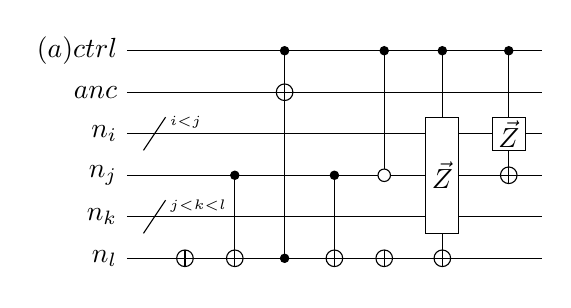
\begin{tikzpicture}[scale=1.000000,x=1pt,y=1pt]
\filldraw[color=white] (0.000000, -7.500000) rectangle (150.000000, 82.500000);
% Drawing wires
% Line 1: c W \text{(a) }ctrl
\draw[color=black] (0.000000,75.000000) -- (150.000000,75.000000);
\draw[color=black] (0.000000,75.000000) node[left] {$\text{(a) }ctrl$};
% Line 2: a W anc
\draw[color=black] (0.000000,60.000000) -- (150.000000,60.000000);
\draw[color=black] (0.000000,60.000000) node[left] {$anc$};
% Line 3: i W n_i
\draw[color=black] (0.000000,45.000000) -- (150.000000,45.000000);
\draw[color=black] (0.000000,45.000000) node[left] {$n_i$};
% Line 4: j W n_j
\draw[color=black] (0.000000,30.000000) -- (150.000000,30.000000);
\draw[color=black] (0.000000,30.000000) node[left] {$n_j$};
% Line 5: k W n_k
\draw[color=black] (0.000000,15.000000) -- (150.000000,15.000000);
\draw[color=black] (0.000000,15.000000) node[left] {$n_k$};
% Line 6: l W n_l
\draw[color=black] (0.000000,0.000000) -- (150.000000,0.000000);
\draw[color=black] (0.000000,0.000000) node[left] {$n_l$};
% Done with wires; drawing gates
% Line 8: i / ^{i<j}
\draw (6.000000, 39.000000) -- (14.000000, 51.000000);
\draw (12.000000, 48.000000) node[right] {$\scriptstyle{^{i<j}}$};
% Line 9: k / ^{j<k<l}
\draw (6.000000, 9.000000) -- (14.000000, 21.000000);
\draw (12.000000, 18.000000) node[right] {$\scriptstyle{^{j<k<l}}$};
% Line 10: c a i j k l LABEL width=-20
% Line 12: +l
\begin{scope}
\draw[fill=white] (21.000000, 0.000000) circle(3.000000pt);
\clip (21.000000, 0.000000) circle(3.000000pt);
\draw (18.000000, 0.000000) -- (24.000000, 0.000000);
\draw (21.000000, -3.000000) -- (21.000000, 3.000000);
\end{scope}
% Line 13: j +l
\draw (39.000000,30.000000) -- (39.000000,0.000000);
\filldraw (39.000000, 30.000000) circle(1.500000pt);
\begin{scope}
\draw[fill=white] (39.000000, 0.000000) circle(3.000000pt);
\clip (39.000000, 0.000000) circle(3.000000pt);
\draw (36.000000, 0.000000) -- (42.000000, 0.000000);
\draw (39.000000, -3.000000) -- (39.000000, 3.000000);
\end{scope}
% Line 14: c l +a
\draw (57.000000,75.000000) -- (57.000000,0.000000);
\filldraw (57.000000, 75.000000) circle(1.500000pt);
\filldraw (57.000000, 0.000000) circle(1.500000pt);
\begin{scope}
\draw[fill=white] (57.000000, 60.000000) circle(3.000000pt);
\clip (57.000000, 60.000000) circle(3.000000pt);
\draw (54.000000, 60.000000) -- (60.000000, 60.000000);
\draw (57.000000, 57.000000) -- (57.000000, 63.000000);
\end{scope}
% Line 15: j +l
\draw (75.000000,30.000000) -- (75.000000,0.000000);
\filldraw (75.000000, 30.000000) circle(1.500000pt);
\begin{scope}
\draw[fill=white] (75.000000, 0.000000) circle(3.000000pt);
\clip (75.000000, 0.000000) circle(3.000000pt);
\draw (72.000000, 0.000000) -- (78.000000, 0.000000);
\draw (75.000000, -3.000000) -- (75.000000, 3.000000);
\end{scope}
% Line 16: +l
\begin{scope}
\draw[fill=white] (93.000000, 0.000000) circle(3.000000pt);
\clip (93.000000, 0.000000) circle(3.000000pt);
\draw (90.000000, 0.000000) -- (96.000000, 0.000000);
\draw (93.000000, -3.000000) -- (93.000000, 3.000000);
\end{scope}
% Line 18: c -j
\draw (93.000000,75.000000) -- (93.000000,30.000000);
\filldraw (93.000000, 75.000000) circle(1.500000pt);
\draw[fill=white] (93.000000, 30.000000) circle(2.250000pt);
% Line 20: i j k G $\vec{Z}$ c +l
\draw (114.000000,75.000000) -- (114.000000,0.000000);
\begin{scope}
\draw[fill=white] (114.000000, 30.000000) +(-45.000000:8.485281pt and 29.698485pt) -- +(45.000000:8.485281pt and 29.698485pt) -- +(135.000000:8.485281pt and 29.698485pt) -- +(225.000000:8.485281pt and 29.698485pt) -- cycle;
\clip (114.000000, 30.000000) +(-45.000000:8.485281pt and 29.698485pt) -- +(45.000000:8.485281pt and 29.698485pt) -- +(135.000000:8.485281pt and 29.698485pt) -- +(225.000000:8.485281pt and 29.698485pt) -- cycle;
\draw (114.000000, 30.000000) node {$\vec{Z}$};
\end{scope}
\filldraw (114.000000, 75.000000) circle(1.500000pt);
\begin{scope}
\draw[fill=white] (114.000000, 0.000000) circle(3.000000pt);
\clip (114.000000, 0.000000) circle(3.000000pt);
\draw (111.000000, 0.000000) -- (117.000000, 0.000000);
\draw (114.000000, -3.000000) -- (114.000000, 3.000000);
\end{scope}
% Line 21: i G $\vec{Z}$ c +j
\draw (138.000000,75.000000) -- (138.000000,30.000000);
\begin{scope}
\draw[fill=white] (138.000000, 45.000000) +(-45.000000:8.485281pt and 8.485281pt) -- +(45.000000:8.485281pt and 8.485281pt) -- +(135.000000:8.485281pt and 8.485281pt) -- +(225.000000:8.485281pt and 8.485281pt) -- cycle;
\clip (138.000000, 45.000000) +(-45.000000:8.485281pt and 8.485281pt) -- +(45.000000:8.485281pt and 8.485281pt) -- +(135.000000:8.485281pt and 8.485281pt) -- +(225.000000:8.485281pt and 8.485281pt) -- cycle;
\draw (138.000000, 45.000000) node {$\vec{Z}$};
\end{scope}
\filldraw (138.000000, 75.000000) circle(1.500000pt);
\begin{scope}
\draw[fill=white] (138.000000, 30.000000) circle(3.000000pt);
\clip (138.000000, 30.000000) circle(3.000000pt);
\draw (135.000000, 30.000000) -- (141.000000, 30.000000);
\draw (138.000000, 27.000000) -- (138.000000, 33.000000);
\end{scope}
% Done with gates; drawing ending labels
% Done with ending labels; drawing cut lines and comments
% Done with comments
\end{tikzpicture}

    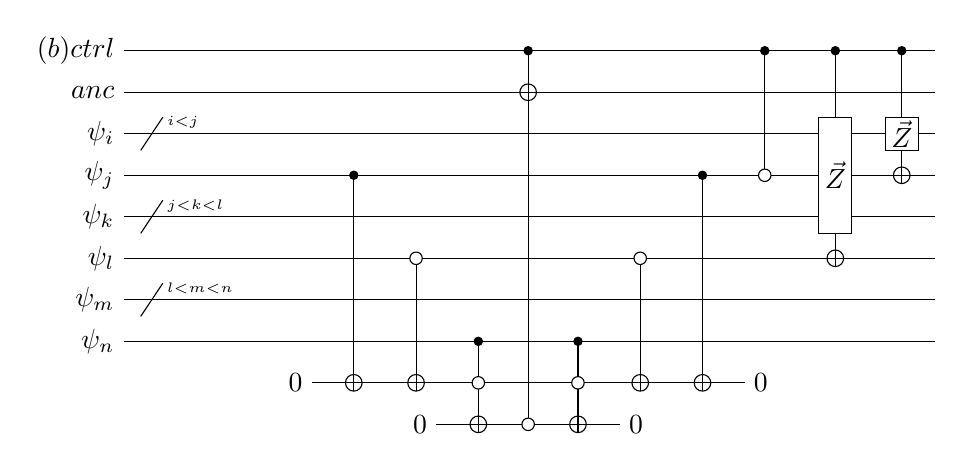
\begin{tikzpicture}[scale=1.000000,x=1pt,y=1pt]
\filldraw[color=white] (0.000000, -7.500000) rectangle (293.000000, 142.500000);
% Drawing wires
% Line 1: c W \text{(b) }ctrl
\draw[color=black] (0.000000,135.000000) -- (293.000000,135.000000);
\draw[color=black] (0.000000,135.000000) node[left] {$\text{(b) }ctrl$};
% Line 2: a W anc
\draw[color=black] (0.000000,120.000000) -- (293.000000,120.000000);
\draw[color=black] (0.000000,120.000000) node[left] {$anc$};
% Line 3: i W \psi_i
\draw[color=black] (0.000000,105.000000) -- (293.000000,105.000000);
\draw[color=black] (0.000000,105.000000) node[left] {$\psi_i$};
% Line 4: j W \psi_j
\draw[color=black] (0.000000,90.000000) -- (293.000000,90.000000);
\draw[color=black] (0.000000,90.000000) node[left] {$\psi_j$};
% Line 5: k W \psi_k
\draw[color=black] (0.000000,75.000000) -- (293.000000,75.000000);
\draw[color=black] (0.000000,75.000000) node[left] {$\psi_k$};
% Line 6: l W \psi_l
\draw[color=black] (0.000000,60.000000) -- (293.000000,60.000000);
\draw[color=black] (0.000000,60.000000) node[left] {$\psi_l$};
% Line 7: m W \psi_m
\draw[color=black] (0.000000,45.000000) -- (293.000000,45.000000);
\draw[color=black] (0.000000,45.000000) node[left] {$\psi_m$};
% Line 8: n W \psi_n
\draw[color=black] (0.000000,30.000000) -- (293.000000,30.000000);
\draw[color=black] (0.000000,30.000000) node[left] {$\psi_n$};
% Line 9: c0 W 0 0
\draw[color=black] (60.500000,15.000000) -- (231.500000,15.000000);
% Line 10: c1 W 0 0
\draw[color=black] (105.500000,0.000000) -- (186.500000,0.000000);
% Done with wires; drawing gates
% Line 12: i / ^{i<j}
\draw (6.000000, 99.000000) -- (14.000000, 111.000000);
\draw (12.000000, 108.000000) node[right] {$\scriptstyle{^{i<j}}$};
% Line 13: k / ^{j<k<l}
\draw (6.000000, 69.000000) -- (14.000000, 81.000000);
\draw (12.000000, 78.000000) node[right] {$\scriptstyle{^{j<k<l}}$};
% Line 14: m / ^{l<m<n}
\draw (6.000000, 39.000000) -- (14.000000, 51.000000);
\draw (12.000000, 48.000000) node[right] {$\scriptstyle{^{l<m<n}}$};
% Line 15: c a i j k l m n c0 c1 LABEL
% Line 16: c0 START
\draw[color=black] (68.000000,15.000000) node[fill=white,left,minimum height=15.000000pt,minimum width=15.000000pt,inner sep=0pt] {\phantom{$0$}};
\draw[color=black] (68.000000,15.000000) node[left] {$0$};
% Line 17: j +c0
\draw (83.000000,90.000000) -- (83.000000,15.000000);
\filldraw (83.000000, 90.000000) circle(1.500000pt);
\begin{scope}
\draw[fill=white] (83.000000, 15.000000) circle(3.000000pt);
\clip (83.000000, 15.000000) circle(3.000000pt);
\draw (80.000000, 15.000000) -- (86.000000, 15.000000);
\draw (83.000000, 12.000000) -- (83.000000, 18.000000);
\end{scope}
% Line 18: -l +c0
\draw (105.500000,60.000000) -- (105.500000,15.000000);
\draw[fill=white] (105.500000, 60.000000) circle(2.250000pt);
\begin{scope}
\draw[fill=white] (105.500000, 15.000000) circle(3.000000pt);
\clip (105.500000, 15.000000) circle(3.000000pt);
\draw (102.500000, 15.000000) -- (108.500000, 15.000000);
\draw (105.500000, 12.000000) -- (105.500000, 18.000000);
\end{scope}
% Line 19: c1 START
\draw[color=black] (113.000000,0.000000) node[fill=white,left,minimum height=15.000000pt,minimum width=15.000000pt,inner sep=0pt] {\phantom{$0$}};
\draw[color=black] (113.000000,0.000000) node[left] {$0$};
% Line 20: n -c0 +c1
\draw (128.000000,30.000000) -- (128.000000,0.000000);
\filldraw (128.000000, 30.000000) circle(1.500000pt);
\draw[fill=white] (128.000000, 15.000000) circle(2.250000pt);
\begin{scope}
\draw[fill=white] (128.000000, 0.000000) circle(3.000000pt);
\clip (128.000000, 0.000000) circle(3.000000pt);
\draw (125.000000, 0.000000) -- (131.000000, 0.000000);
\draw (128.000000, -3.000000) -- (128.000000, 3.000000);
\end{scope}
% Line 21: c -c1 +a
\draw (146.000000,135.000000) -- (146.000000,0.000000);
\filldraw (146.000000, 135.000000) circle(1.500000pt);
\draw[fill=white] (146.000000, 0.000000) circle(2.250000pt);
\begin{scope}
\draw[fill=white] (146.000000, 120.000000) circle(3.000000pt);
\clip (146.000000, 120.000000) circle(3.000000pt);
\draw (143.000000, 120.000000) -- (149.000000, 120.000000);
\draw (146.000000, 117.000000) -- (146.000000, 123.000000);
\end{scope}
% Line 22: n -c0 +c1
\draw (164.000000,30.000000) -- (164.000000,0.000000);
\filldraw (164.000000, 30.000000) circle(1.500000pt);
\draw[fill=white] (164.000000, 15.000000) circle(2.250000pt);
\begin{scope}
\draw[fill=white] (164.000000, 0.000000) circle(3.000000pt);
\clip (164.000000, 0.000000) circle(3.000000pt);
\draw (161.000000, 0.000000) -- (167.000000, 0.000000);
\draw (164.000000, -3.000000) -- (164.000000, 3.000000);
\end{scope}
% Line 23: c1 END
\draw[color=black] (179.000000,0.000000) node[fill=white,right,minimum height=15.000000pt,minimum width=15.000000pt,inner sep=0pt] {\phantom{$0$}};
\draw[color=black] (179.000000,0.000000) node[right] {$0$};
% Line 24: -l +c0
\draw (186.500000,60.000000) -- (186.500000,15.000000);
\draw[fill=white] (186.500000, 60.000000) circle(2.250000pt);
\begin{scope}
\draw[fill=white] (186.500000, 15.000000) circle(3.000000pt);
\clip (186.500000, 15.000000) circle(3.000000pt);
\draw (183.500000, 15.000000) -- (189.500000, 15.000000);
\draw (186.500000, 12.000000) -- (186.500000, 18.000000);
\end{scope}
% Line 25: j +c0
\draw (209.000000,90.000000) -- (209.000000,15.000000);
\filldraw (209.000000, 90.000000) circle(1.500000pt);
\begin{scope}
\draw[fill=white] (209.000000, 15.000000) circle(3.000000pt);
\clip (209.000000, 15.000000) circle(3.000000pt);
\draw (206.000000, 15.000000) -- (212.000000, 15.000000);
\draw (209.000000, 12.000000) -- (209.000000, 18.000000);
\end{scope}
% Line 26: c0 END
\draw[color=black] (224.000000,15.000000) node[fill=white,right,minimum height=15.000000pt,minimum width=15.000000pt,inner sep=0pt] {\phantom{$0$}};
\draw[color=black] (224.000000,15.000000) node[right] {$0$};
% Line 27: c -j
\draw (231.500000,135.000000) -- (231.500000,90.000000);
\filldraw (231.500000, 135.000000) circle(1.500000pt);
\draw[fill=white] (231.500000, 90.000000) circle(2.250000pt);
% Line 29: i j k G $\vec{Z}$ c +l
\draw (257.000000,135.000000) -- (257.000000,60.000000);
\begin{scope}
\draw[fill=white] (257.000000, 90.000000) +(-45.000000:8.485281pt and 29.698485pt) -- +(45.000000:8.485281pt and 29.698485pt) -- +(135.000000:8.485281pt and 29.698485pt) -- +(225.000000:8.485281pt and 29.698485pt) -- cycle;
\clip (257.000000, 90.000000) +(-45.000000:8.485281pt and 29.698485pt) -- +(45.000000:8.485281pt and 29.698485pt) -- +(135.000000:8.485281pt and 29.698485pt) -- +(225.000000:8.485281pt and 29.698485pt) -- cycle;
\draw (257.000000, 90.000000) node {$\vec{Z}$};
\end{scope}
\filldraw (257.000000, 135.000000) circle(1.500000pt);
\begin{scope}
\draw[fill=white] (257.000000, 60.000000) circle(3.000000pt);
\clip (257.000000, 60.000000) circle(3.000000pt);
\draw (254.000000, 60.000000) -- (260.000000, 60.000000);
\draw (257.000000, 57.000000) -- (257.000000, 63.000000);
\end{scope}
% Line 30: i G $\vec{Z}$ c +j
\draw (281.000000,135.000000) -- (281.000000,90.000000);
\begin{scope}
\draw[fill=white] (281.000000, 105.000000) +(-45.000000:8.485281pt and 8.485281pt) -- +(45.000000:8.485281pt and 8.485281pt) -- +(135.000000:8.485281pt and 8.485281pt) -- +(225.000000:8.485281pt and 8.485281pt) -- cycle;
\clip (281.000000, 105.000000) +(-45.000000:8.485281pt and 8.485281pt) -- +(45.000000:8.485281pt and 8.485281pt) -- +(135.000000:8.485281pt and 8.485281pt) -- +(225.000000:8.485281pt and 8.485281pt) -- cycle;
\draw (281.000000, 105.000000) node {$\vec{Z}$};
\end{scope}
\filldraw (281.000000, 135.000000) circle(1.500000pt);
\begin{scope}
\draw[fill=white] (281.000000, 90.000000) circle(3.000000pt);
\clip (281.000000, 90.000000) circle(3.000000pt);
\draw (278.000000, 90.000000) -- (284.000000, 90.000000);
\draw (281.000000, 87.000000) -- (281.000000, 93.000000);
\end{scope}
% Done with gates; drawing ending labels
% Done with ending labels; drawing cut lines and comments
% Done with comments
\end{tikzpicture}

    \caption{
        \textbf{Block-Encoding Product of Fermionic Operators Plus Hermitian Conjugate (modifications)}
        In subfigure a, a block-encoding for the operator $b_j b_l^\dagger + b_l b_j^\dagger$ is given.
        In subfigure b, a block-encoding for the operator $b_j b_l^\dagger b_n^\dagger b_n + b_n^\dagger b_n b_l b_j^\dagger$ is given.
    }
    \label{fig:fermionic-be-lc-modifications}
\end{figure}

For an operator with the form $b_i b_j^\dagger + b_j b_i^\dagger$, we can construct a block-encoding using with a slight modification.
In this case, we compute the variable $\ket{a}$ with the CNOT acting on the $j^\text{th}$ mode being $0$-controlled.
The circuit diagram for block-encoding this operator is given in subfigure \ref{fig:fermionic-be-lc-modifications}a.
Likewise, if a number operator is included in a term, then this can be accounted for by including a $1$-control on that mode when determining if the block-encoding ancilla should be flipped.
An example circuit diagram for an operator including a number operator is given in subfigure \ref{fig:fermionic-be-lc-modifications}b.

\begin{figure}
    \definecolor{tblue}{RGB}{61,142,221}
\definecolor{torange}{RGB}{253,143,41}
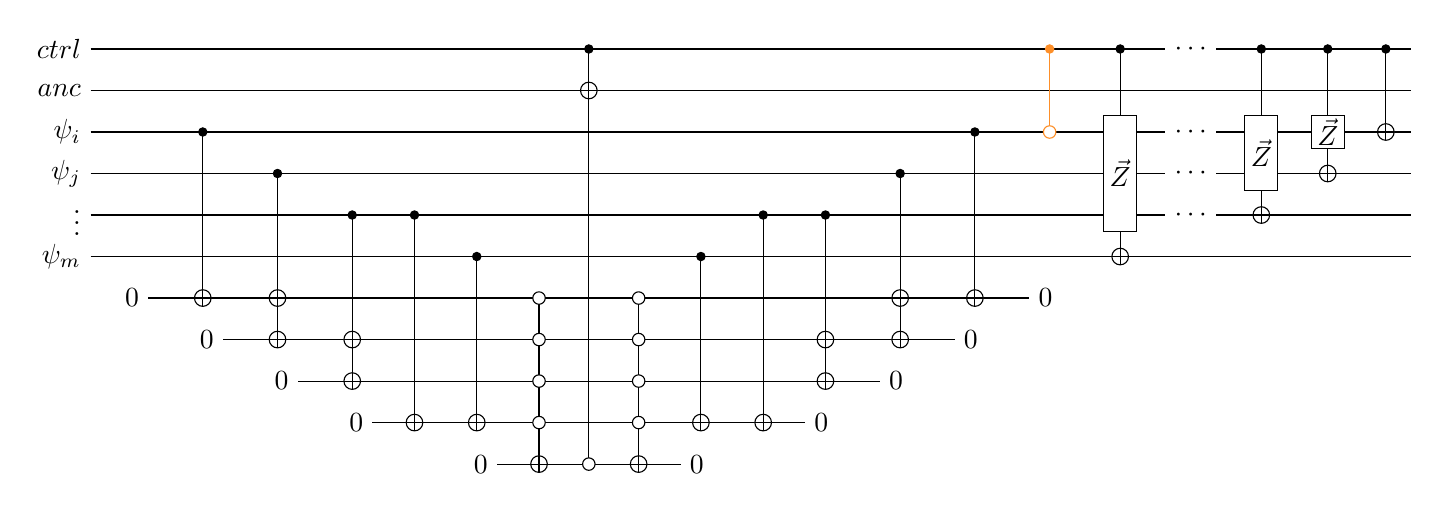
\begin{tikzpicture}[scale=1.000000,x=1pt,y=1pt]
\filldraw[color=white] (0.000000, -7.500000) rectangle (477.000000, 157.500000);
% Drawing wires
% Line 4: ctrl W ctrl
\draw[color=black] (0.000000,150.000000) -- (477.000000,150.000000);
\draw[color=black] (0.000000,150.000000) node[left] {$ctrl$};
% Line 5: anc W anc
\draw[color=black] (0.000000,135.000000) -- (477.000000,135.000000);
\draw[color=black] (0.000000,135.000000) node[left] {$anc$};
% Line 6: a W \psi_i
\draw[color=black] (0.000000,120.000000) -- (477.000000,120.000000);
\draw[color=black] (0.000000,120.000000) node[left] {$\psi_i$};
% Line 7: b W \psi_j
\draw[color=black] (0.000000,105.000000) -- (477.000000,105.000000);
\draw[color=black] (0.000000,105.000000) node[left] {$\psi_j$};
% Line 8: c W \vdots
\draw[color=black] (0.000000,90.000000) -- (477.000000,90.000000);
\draw[color=black] (0.000000,90.000000) node[left] {$\vdots$};
% Line 9: f W \psi_m
\draw[color=black] (0.000000,75.000000) -- (477.000000,75.000000);
\draw[color=black] (0.000000,75.000000) node[left] {$\psi_m$};
% Line 10: c0 W 0 0
\draw[color=black] (13.500000,60.000000) -- (346.500000,60.000000);
% Line 11: c1 W 0 0
\draw[color=black] (40.500000,45.000000) -- (319.500000,45.000000);
% Line 12: c2 W 0 0
\draw[color=black] (67.500000,30.000000) -- (292.500000,30.000000);
% Line 13: 1 W 0 0
\draw[color=black] (94.500000,15.000000) -- (265.500000,15.000000);
% Line 14: c3 W 0 0
\draw[color=black] (139.500000,0.000000) -- (220.500000,0.000000);
% Done with wires; drawing gates
% Line 16: c0 START
\draw[color=black] (21.000000,60.000000) node[fill=white,left,minimum height=15.000000pt,minimum width=15.000000pt,inner sep=0pt] {\phantom{$0$}};
\draw[color=black] (21.000000,60.000000) node[left] {$0$};
% Line 17: a +c0
\draw (40.500000,120.000000) -- (40.500000,60.000000);
\filldraw (40.500000, 120.000000) circle(1.500000pt);
\begin{scope}
\draw[fill=white] (40.500000, 60.000000) circle(3.000000pt);
\clip (40.500000, 60.000000) circle(3.000000pt);
\draw (37.500000, 60.000000) -- (43.500000, 60.000000);
\draw (40.500000, 57.000000) -- (40.500000, 63.000000);
\end{scope}
% Line 18: c1 START
\draw[color=black] (48.000000,45.000000) node[fill=white,left,minimum height=15.000000pt,minimum width=15.000000pt,inner sep=0pt] {\phantom{$0$}};
\draw[color=black] (48.000000,45.000000) node[left] {$0$};
% Line 19: b +c0 +c1
\draw (67.500000,105.000000) -- (67.500000,45.000000);
\filldraw (67.500000, 105.000000) circle(1.500000pt);
\begin{scope}
\draw[fill=white] (67.500000, 60.000000) circle(3.000000pt);
\clip (67.500000, 60.000000) circle(3.000000pt);
\draw (64.500000, 60.000000) -- (70.500000, 60.000000);
\draw (67.500000, 57.000000) -- (67.500000, 63.000000);
\end{scope}
\begin{scope}
\draw[fill=white] (67.500000, 45.000000) circle(3.000000pt);
\clip (67.500000, 45.000000) circle(3.000000pt);
\draw (64.500000, 45.000000) -- (70.500000, 45.000000);
\draw (67.500000, 42.000000) -- (67.500000, 48.000000);
\end{scope}
% Line 20: c2 START
\draw[color=black] (75.000000,30.000000) node[fill=white,left,minimum height=15.000000pt,minimum width=15.000000pt,inner sep=0pt] {\phantom{$0$}};
\draw[color=black] (75.000000,30.000000) node[left] {$0$};
% Line 21: c +c1 +c2
\draw (94.500000,90.000000) -- (94.500000,30.000000);
\filldraw (94.500000, 90.000000) circle(1.500000pt);
\begin{scope}
\draw[fill=white] (94.500000, 45.000000) circle(3.000000pt);
\clip (94.500000, 45.000000) circle(3.000000pt);
\draw (91.500000, 45.000000) -- (97.500000, 45.000000);
\draw (94.500000, 42.000000) -- (94.500000, 48.000000);
\end{scope}
\begin{scope}
\draw[fill=white] (94.500000, 30.000000) circle(3.000000pt);
\clip (94.500000, 30.000000) circle(3.000000pt);
\draw (91.500000, 30.000000) -- (97.500000, 30.000000);
\draw (94.500000, 27.000000) -- (94.500000, 33.000000);
\end{scope}
% Line 22: 1 START
\draw[color=black] (102.000000,15.000000) node[fill=white,left,minimum height=15.000000pt,minimum width=15.000000pt,inner sep=0pt] {\phantom{$0$}};
\draw[color=black] (102.000000,15.000000) node[left] {$0$};
% Line 23: c +1
\draw (117.000000,90.000000) -- (117.000000,15.000000);
\filldraw (117.000000, 90.000000) circle(1.500000pt);
\begin{scope}
\draw[fill=white] (117.000000, 15.000000) circle(3.000000pt);
\clip (117.000000, 15.000000) circle(3.000000pt);
\draw (114.000000, 15.000000) -- (120.000000, 15.000000);
\draw (117.000000, 12.000000) -- (117.000000, 18.000000);
\end{scope}
% Line 24: f +1
\draw (139.500000,75.000000) -- (139.500000,15.000000);
\filldraw (139.500000, 75.000000) circle(1.500000pt);
\begin{scope}
\draw[fill=white] (139.500000, 15.000000) circle(3.000000pt);
\clip (139.500000, 15.000000) circle(3.000000pt);
\draw (136.500000, 15.000000) -- (142.500000, 15.000000);
\draw (139.500000, 12.000000) -- (139.500000, 18.000000);
\end{scope}
% Line 26: c3 START
\draw[color=black] (147.000000,0.000000) node[fill=white,left,minimum height=15.000000pt,minimum width=15.000000pt,inner sep=0pt] {\phantom{$0$}};
\draw[color=black] (147.000000,0.000000) node[left] {$0$};
% Line 27: -c0 -c1 -c2 -1 +c3
\draw (162.000000,60.000000) -- (162.000000,0.000000);
\draw[fill=white] (162.000000, 60.000000) circle(2.250000pt);
\draw[fill=white] (162.000000, 45.000000) circle(2.250000pt);
\draw[fill=white] (162.000000, 30.000000) circle(2.250000pt);
\draw[fill=white] (162.000000, 15.000000) circle(2.250000pt);
\begin{scope}
\draw[fill=white] (162.000000, 0.000000) circle(3.000000pt);
\clip (162.000000, 0.000000) circle(3.000000pt);
\draw (159.000000, 0.000000) -- (165.000000, 0.000000);
\draw (162.000000, -3.000000) -- (162.000000, 3.000000);
\end{scope}
% Line 28: ctrl -c3 +anc
\draw (180.000000,150.000000) -- (180.000000,0.000000);
\filldraw (180.000000, 150.000000) circle(1.500000pt);
\draw[fill=white] (180.000000, 0.000000) circle(2.250000pt);
\begin{scope}
\draw[fill=white] (180.000000, 135.000000) circle(3.000000pt);
\clip (180.000000, 135.000000) circle(3.000000pt);
\draw (177.000000, 135.000000) -- (183.000000, 135.000000);
\draw (180.000000, 132.000000) -- (180.000000, 138.000000);
\end{scope}
% Line 29: -c0 -c1 -c2 -1 +c3
\draw (198.000000,60.000000) -- (198.000000,0.000000);
\draw[fill=white] (198.000000, 60.000000) circle(2.250000pt);
\draw[fill=white] (198.000000, 45.000000) circle(2.250000pt);
\draw[fill=white] (198.000000, 30.000000) circle(2.250000pt);
\draw[fill=white] (198.000000, 15.000000) circle(2.250000pt);
\begin{scope}
\draw[fill=white] (198.000000, 0.000000) circle(3.000000pt);
\clip (198.000000, 0.000000) circle(3.000000pt);
\draw (195.000000, 0.000000) -- (201.000000, 0.000000);
\draw (198.000000, -3.000000) -- (198.000000, 3.000000);
\end{scope}
% Line 30: c3 END
\draw[color=black] (213.000000,0.000000) node[fill=white,right,minimum height=15.000000pt,minimum width=15.000000pt,inner sep=0pt] {\phantom{$0$}};
\draw[color=black] (213.000000,0.000000) node[right] {$0$};
% Line 32: f +1
\draw (220.500000,75.000000) -- (220.500000,15.000000);
\filldraw (220.500000, 75.000000) circle(1.500000pt);
\begin{scope}
\draw[fill=white] (220.500000, 15.000000) circle(3.000000pt);
\clip (220.500000, 15.000000) circle(3.000000pt);
\draw (217.500000, 15.000000) -- (223.500000, 15.000000);
\draw (220.500000, 12.000000) -- (220.500000, 18.000000);
\end{scope}
% Line 33: c +1
\draw (243.000000,90.000000) -- (243.000000,15.000000);
\filldraw (243.000000, 90.000000) circle(1.500000pt);
\begin{scope}
\draw[fill=white] (243.000000, 15.000000) circle(3.000000pt);
\clip (243.000000, 15.000000) circle(3.000000pt);
\draw (240.000000, 15.000000) -- (246.000000, 15.000000);
\draw (243.000000, 12.000000) -- (243.000000, 18.000000);
\end{scope}
% Line 34: 1 END
\draw[color=black] (258.000000,15.000000) node[fill=white,right,minimum height=15.000000pt,minimum width=15.000000pt,inner sep=0pt] {\phantom{$0$}};
\draw[color=black] (258.000000,15.000000) node[right] {$0$};
% Line 35: c +c1 +c2
\draw (265.500000,90.000000) -- (265.500000,30.000000);
\filldraw (265.500000, 90.000000) circle(1.500000pt);
\begin{scope}
\draw[fill=white] (265.500000, 45.000000) circle(3.000000pt);
\clip (265.500000, 45.000000) circle(3.000000pt);
\draw (262.500000, 45.000000) -- (268.500000, 45.000000);
\draw (265.500000, 42.000000) -- (265.500000, 48.000000);
\end{scope}
\begin{scope}
\draw[fill=white] (265.500000, 30.000000) circle(3.000000pt);
\clip (265.500000, 30.000000) circle(3.000000pt);
\draw (262.500000, 30.000000) -- (268.500000, 30.000000);
\draw (265.500000, 27.000000) -- (265.500000, 33.000000);
\end{scope}
% Line 36: c2 END
\draw[color=black] (285.000000,30.000000) node[fill=white,right,minimum height=15.000000pt,minimum width=15.000000pt,inner sep=0pt] {\phantom{$0$}};
\draw[color=black] (285.000000,30.000000) node[right] {$0$};
% Line 37: b +c0 +c1
\draw (292.500000,105.000000) -- (292.500000,45.000000);
\filldraw (292.500000, 105.000000) circle(1.500000pt);
\begin{scope}
\draw[fill=white] (292.500000, 60.000000) circle(3.000000pt);
\clip (292.500000, 60.000000) circle(3.000000pt);
\draw (289.500000, 60.000000) -- (295.500000, 60.000000);
\draw (292.500000, 57.000000) -- (292.500000, 63.000000);
\end{scope}
\begin{scope}
\draw[fill=white] (292.500000, 45.000000) circle(3.000000pt);
\clip (292.500000, 45.000000) circle(3.000000pt);
\draw (289.500000, 45.000000) -- (295.500000, 45.000000);
\draw (292.500000, 42.000000) -- (292.500000, 48.000000);
\end{scope}
% Line 38: c1 END
\draw[color=black] (312.000000,45.000000) node[fill=white,right,minimum height=15.000000pt,minimum width=15.000000pt,inner sep=0pt] {\phantom{$0$}};
\draw[color=black] (312.000000,45.000000) node[right] {$0$};
% Line 39: a +c0
\draw (319.500000,120.000000) -- (319.500000,60.000000);
\filldraw (319.500000, 120.000000) circle(1.500000pt);
\begin{scope}
\draw[fill=white] (319.500000, 60.000000) circle(3.000000pt);
\clip (319.500000, 60.000000) circle(3.000000pt);
\draw (316.500000, 60.000000) -- (322.500000, 60.000000);
\draw (319.500000, 57.000000) -- (319.500000, 63.000000);
\end{scope}
% Line 40: c0 END
\draw[color=black] (339.000000,60.000000) node[fill=white,right,minimum height=15.000000pt,minimum width=15.000000pt,inner sep=0pt] {\phantom{$0$}};
\draw[color=black] (339.000000,60.000000) node[right] {$0$};
% Line 44: ctrl -a color=torange
\begin{scope}[color=torange]
\draw (346.500000,150.000000) -- (346.500000,120.000000);
\filldraw (346.500000, 150.000000) circle(1.500000pt);
\draw[fill=white] (346.500000, 120.000000) circle(2.250000pt);
\end{scope}
% Line 46: a b c G $\vec{Z}$ ctrl +f
\draw (372.000000,150.000000) -- (372.000000,75.000000);
\begin{scope}
\draw[fill=white] (372.000000, 105.000000) +(-45.000000:8.485281pt and 29.698485pt) -- +(45.000000:8.485281pt and 29.698485pt) -- +(135.000000:8.485281pt and 29.698485pt) -- +(225.000000:8.485281pt and 29.698485pt) -- cycle;
\clip (372.000000, 105.000000) +(-45.000000:8.485281pt and 29.698485pt) -- +(45.000000:8.485281pt and 29.698485pt) -- +(135.000000:8.485281pt and 29.698485pt) -- +(225.000000:8.485281pt and 29.698485pt) -- cycle;
\draw (372.000000, 105.000000) node {$\vec{Z}$};
\end{scope}
\filldraw (372.000000, 150.000000) circle(1.500000pt);
\begin{scope}
\draw[fill=white] (372.000000, 75.000000) circle(3.000000pt);
\clip (372.000000, 75.000000) circle(3.000000pt);
\draw (369.000000, 75.000000) -- (375.000000, 75.000000);
\draw (372.000000, 72.000000) -- (372.000000, 78.000000);
\end{scope}
% Line 47: ctrl a b c LABEL ...
\draw[color=black] (397.500000, 150.000000) node [fill=white] {$\cdots$};
\draw[color=black] (397.500000, 120.000000) node [fill=white] {$\cdots$};
\draw[color=black] (397.500000, 105.000000) node [fill=white] {$\cdots$};
\draw[color=black] (397.500000, 90.000000) node [fill=white] {$\cdots$};
% Line 48: a b G $\vec{Z}$ ctrl +c
\draw (423.000000,150.000000) -- (423.000000,90.000000);
\begin{scope}
\draw[fill=white] (423.000000, 112.500000) +(-45.000000:8.485281pt and 19.091883pt) -- +(45.000000:8.485281pt and 19.091883pt) -- +(135.000000:8.485281pt and 19.091883pt) -- +(225.000000:8.485281pt and 19.091883pt) -- cycle;
\clip (423.000000, 112.500000) +(-45.000000:8.485281pt and 19.091883pt) -- +(45.000000:8.485281pt and 19.091883pt) -- +(135.000000:8.485281pt and 19.091883pt) -- +(225.000000:8.485281pt and 19.091883pt) -- cycle;
\draw (423.000000, 112.500000) node {$\vec{Z}$};
\end{scope}
\filldraw (423.000000, 150.000000) circle(1.500000pt);
\begin{scope}
\draw[fill=white] (423.000000, 90.000000) circle(3.000000pt);
\clip (423.000000, 90.000000) circle(3.000000pt);
\draw (420.000000, 90.000000) -- (426.000000, 90.000000);
\draw (423.000000, 87.000000) -- (423.000000, 93.000000);
\end{scope}
% Line 49: a G $\vec{Z}$ ctrl +b
\draw (447.000000,150.000000) -- (447.000000,105.000000);
\begin{scope}
\draw[fill=white] (447.000000, 120.000000) +(-45.000000:8.485281pt and 8.485281pt) -- +(45.000000:8.485281pt and 8.485281pt) -- +(135.000000:8.485281pt and 8.485281pt) -- +(225.000000:8.485281pt and 8.485281pt) -- cycle;
\clip (447.000000, 120.000000) +(-45.000000:8.485281pt and 8.485281pt) -- +(45.000000:8.485281pt and 8.485281pt) -- +(135.000000:8.485281pt and 8.485281pt) -- +(225.000000:8.485281pt and 8.485281pt) -- cycle;
\draw (447.000000, 120.000000) node {$\vec{Z}$};
\end{scope}
\filldraw (447.000000, 150.000000) circle(1.500000pt);
\begin{scope}
\draw[fill=white] (447.000000, 105.000000) circle(3.000000pt);
\clip (447.000000, 105.000000) circle(3.000000pt);
\draw (444.000000, 105.000000) -- (450.000000, 105.000000);
\draw (447.000000, 102.000000) -- (447.000000, 108.000000);
\end{scope}
% Line 50: ctrl +a
\draw (468.000000,150.000000) -- (468.000000,120.000000);
\filldraw (468.000000, 150.000000) circle(1.500000pt);
\begin{scope}
\draw[fill=white] (468.000000, 120.000000) circle(3.000000pt);
\clip (468.000000, 120.000000) circle(3.000000pt);
\draw (465.000000, 120.000000) -- (471.000000, 120.000000);
\draw (468.000000, 117.000000) -- (468.000000, 123.000000);
\end{scope}
% Done with gates; drawing ending labels
% Done with ending labels; drawing cut lines and comments
% Done with comments
\end{tikzpicture}

    \caption{
        \textbf{Generalized Block-Encoding for Product of Fermionic Operators Plus Hermitian Conjugate}
        A block-encoding for the operator $b_i b_j ... b_m + b_m^\dagger ... b_j^\dagger b_i^\dagger$ is given.
        The $CZ$ gate highlighted in orange is present if $C \text{ choose } 2$ is odd where $C$ is the number of active modes excluding modes with number operators acting on them.
        Block-encodings for similar operators such as those that include number operators or different arrangements of the creation and annihilation operators can be accounted for using the modifications shown in Figure \ref{fig:fermionic-be-lc-modifications}.
    }
    \label{fig:fermionic-be-lc}
\end{figure}

The construction of these block-encoding circuits can be generalized to any operator that is a product of fermionic operators plus its hermitian conjugate.
An example circuit diagram for this generalized construction is shown in Figure \ref{fig:fermionic-be-lc}.
The $CZ$ gate that applies the sign flip on the second term that can occur when the order of the fermionic operators is swapped is only present if the number of swaps is odd.
If $C$ represents the number of active modes excluding modes where a number operator is acting on the mode, then the number of required swaps is $C \text{ choose } 2$.
In general, these block-encoding circuits will all have optimal rescaling factors ($\lambda=1$), require one block-encoding ancilla, and use $B-1$ Toffoli gates where $B$ is the number of active modes in the operator.

\begin{figure}
    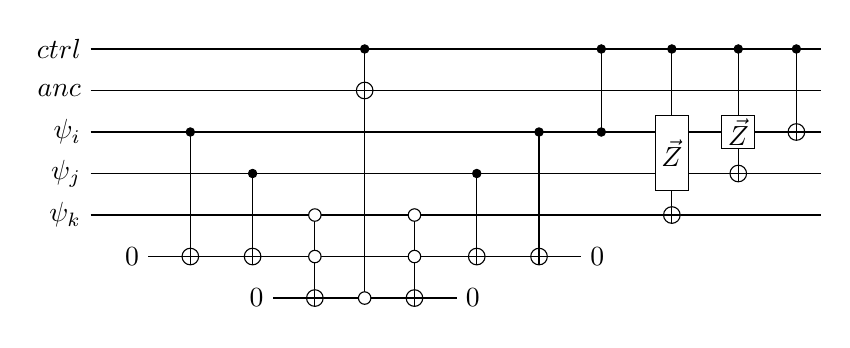
\begin{tikzpicture}[scale=1.000000,x=1pt,y=1pt]
\filldraw[color=white] (0.000000, -7.500000) rectangle (264.000000, 97.500000);
% Drawing wires
% Line 1: ctrl W ctrl
\draw[color=black] (0.000000,90.000000) -- (264.000000,90.000000);
\draw[color=black] (0.000000,90.000000) node[left] {$ctrl$};
% Line 2: anc W anc
\draw[color=black] (0.000000,75.000000) -- (264.000000,75.000000);
\draw[color=black] (0.000000,75.000000) node[left] {$anc$};
% Line 3: i W \psi_i
\draw[color=black] (0.000000,60.000000) -- (264.000000,60.000000);
\draw[color=black] (0.000000,60.000000) node[left] {$\psi_i$};
% Line 4: j W \psi_j
\draw[color=black] (0.000000,45.000000) -- (264.000000,45.000000);
\draw[color=black] (0.000000,45.000000) node[left] {$\psi_j$};
% Line 5: k W \psi_k
\draw[color=black] (0.000000,30.000000) -- (264.000000,30.000000);
\draw[color=black] (0.000000,30.000000) node[left] {$\psi_k$};
% Line 6: c0 W 0 0
\draw[color=black] (13.500000,15.000000) -- (184.500000,15.000000);
% Line 7: c1 W 0 0
\draw[color=black] (58.500000,0.000000) -- (139.500000,0.000000);
% Done with wires; drawing gates
% Line 9: c0 START
\draw[color=black] (21.000000,15.000000) node[fill=white,left,minimum height=15.000000pt,minimum width=15.000000pt,inner sep=0pt] {\phantom{$0$}};
\draw[color=black] (21.000000,15.000000) node[left] {$0$};
% Line 10: i +c0
\draw (36.000000,60.000000) -- (36.000000,15.000000);
\filldraw (36.000000, 60.000000) circle(1.500000pt);
\begin{scope}
\draw[fill=white] (36.000000, 15.000000) circle(3.000000pt);
\clip (36.000000, 15.000000) circle(3.000000pt);
\draw (33.000000, 15.000000) -- (39.000000, 15.000000);
\draw (36.000000, 12.000000) -- (36.000000, 18.000000);
\end{scope}
% Line 11: j +c0
\draw (58.500000,45.000000) -- (58.500000,15.000000);
\filldraw (58.500000, 45.000000) circle(1.500000pt);
\begin{scope}
\draw[fill=white] (58.500000, 15.000000) circle(3.000000pt);
\clip (58.500000, 15.000000) circle(3.000000pt);
\draw (55.500000, 15.000000) -- (61.500000, 15.000000);
\draw (58.500000, 12.000000) -- (58.500000, 18.000000);
\end{scope}
% Line 12: c1 START
\draw[color=black] (66.000000,0.000000) node[fill=white,left,minimum height=15.000000pt,minimum width=15.000000pt,inner sep=0pt] {\phantom{$0$}};
\draw[color=black] (66.000000,0.000000) node[left] {$0$};
% Line 13: -k -c0 +c1
\draw (81.000000,30.000000) -- (81.000000,0.000000);
\draw[fill=white] (81.000000, 30.000000) circle(2.250000pt);
\draw[fill=white] (81.000000, 15.000000) circle(2.250000pt);
\begin{scope}
\draw[fill=white] (81.000000, 0.000000) circle(3.000000pt);
\clip (81.000000, 0.000000) circle(3.000000pt);
\draw (78.000000, 0.000000) -- (84.000000, 0.000000);
\draw (81.000000, -3.000000) -- (81.000000, 3.000000);
\end{scope}
% Line 14: ctrl -c1 +anc
\draw (99.000000,90.000000) -- (99.000000,0.000000);
\filldraw (99.000000, 90.000000) circle(1.500000pt);
\draw[fill=white] (99.000000, 0.000000) circle(2.250000pt);
\begin{scope}
\draw[fill=white] (99.000000, 75.000000) circle(3.000000pt);
\clip (99.000000, 75.000000) circle(3.000000pt);
\draw (96.000000, 75.000000) -- (102.000000, 75.000000);
\draw (99.000000, 72.000000) -- (99.000000, 78.000000);
\end{scope}
% Line 15: -k -c0 +c1
\draw (117.000000,30.000000) -- (117.000000,0.000000);
\draw[fill=white] (117.000000, 30.000000) circle(2.250000pt);
\draw[fill=white] (117.000000, 15.000000) circle(2.250000pt);
\begin{scope}
\draw[fill=white] (117.000000, 0.000000) circle(3.000000pt);
\clip (117.000000, 0.000000) circle(3.000000pt);
\draw (114.000000, 0.000000) -- (120.000000, 0.000000);
\draw (117.000000, -3.000000) -- (117.000000, 3.000000);
\end{scope}
% Line 16: c1 END
\draw[color=black] (132.000000,0.000000) node[fill=white,right,minimum height=15.000000pt,minimum width=15.000000pt,inner sep=0pt] {\phantom{$0$}};
\draw[color=black] (132.000000,0.000000) node[right] {$0$};
% Line 17: j +c0
\draw (139.500000,45.000000) -- (139.500000,15.000000);
\filldraw (139.500000, 45.000000) circle(1.500000pt);
\begin{scope}
\draw[fill=white] (139.500000, 15.000000) circle(3.000000pt);
\clip (139.500000, 15.000000) circle(3.000000pt);
\draw (136.500000, 15.000000) -- (142.500000, 15.000000);
\draw (139.500000, 12.000000) -- (139.500000, 18.000000);
\end{scope}
% Line 18: i +c0
\draw (162.000000,60.000000) -- (162.000000,15.000000);
\filldraw (162.000000, 60.000000) circle(1.500000pt);
\begin{scope}
\draw[fill=white] (162.000000, 15.000000) circle(3.000000pt);
\clip (162.000000, 15.000000) circle(3.000000pt);
\draw (159.000000, 15.000000) -- (165.000000, 15.000000);
\draw (162.000000, 12.000000) -- (162.000000, 18.000000);
\end{scope}
% Line 19: c0 END
\draw[color=black] (177.000000,15.000000) node[fill=white,right,minimum height=15.000000pt,minimum width=15.000000pt,inner sep=0pt] {\phantom{$0$}};
\draw[color=black] (177.000000,15.000000) node[right] {$0$};
% Line 21: ctrl i
\draw (184.500000,90.000000) -- (184.500000,60.000000);
\filldraw (184.500000, 90.000000) circle(1.500000pt);
\filldraw (184.500000, 60.000000) circle(1.500000pt);
% Line 23: i j G $\vec{Z}$ ctrl +k
\draw (210.000000,90.000000) -- (210.000000,30.000000);
\begin{scope}
\draw[fill=white] (210.000000, 52.500000) +(-45.000000:8.485281pt and 19.091883pt) -- +(45.000000:8.485281pt and 19.091883pt) -- +(135.000000:8.485281pt and 19.091883pt) -- +(225.000000:8.485281pt and 19.091883pt) -- cycle;
\clip (210.000000, 52.500000) +(-45.000000:8.485281pt and 19.091883pt) -- +(45.000000:8.485281pt and 19.091883pt) -- +(135.000000:8.485281pt and 19.091883pt) -- +(225.000000:8.485281pt and 19.091883pt) -- cycle;
\draw (210.000000, 52.500000) node {$\vec{Z}$};
\end{scope}
\filldraw (210.000000, 90.000000) circle(1.500000pt);
\begin{scope}
\draw[fill=white] (210.000000, 30.000000) circle(3.000000pt);
\clip (210.000000, 30.000000) circle(3.000000pt);
\draw (207.000000, 30.000000) -- (213.000000, 30.000000);
\draw (210.000000, 27.000000) -- (210.000000, 33.000000);
\end{scope}
% Line 24: i G $\vec{Z}$ ctrl +j
\draw (234.000000,90.000000) -- (234.000000,45.000000);
\begin{scope}
\draw[fill=white] (234.000000, 60.000000) +(-45.000000:8.485281pt and 8.485281pt) -- +(45.000000:8.485281pt and 8.485281pt) -- +(135.000000:8.485281pt and 8.485281pt) -- +(225.000000:8.485281pt and 8.485281pt) -- cycle;
\clip (234.000000, 60.000000) +(-45.000000:8.485281pt and 8.485281pt) -- +(45.000000:8.485281pt and 8.485281pt) -- +(135.000000:8.485281pt and 8.485281pt) -- +(225.000000:8.485281pt and 8.485281pt) -- cycle;
\draw (234.000000, 60.000000) node {$\vec{Z}$};
\end{scope}
\filldraw (234.000000, 90.000000) circle(1.500000pt);
\begin{scope}
\draw[fill=white] (234.000000, 45.000000) circle(3.000000pt);
\clip (234.000000, 45.000000) circle(3.000000pt);
\draw (231.000000, 45.000000) -- (237.000000, 45.000000);
\draw (234.000000, 42.000000) -- (234.000000, 48.000000);
\end{scope}
% Line 25: ctrl +i
\draw (255.000000,90.000000) -- (255.000000,60.000000);
\filldraw (255.000000, 90.000000) circle(1.500000pt);
\begin{scope}
\draw[fill=white] (255.000000, 60.000000) circle(3.000000pt);
\clip (255.000000, 60.000000) circle(3.000000pt);
\draw (252.000000, 60.000000) -- (258.000000, 60.000000);
\draw (255.000000, 57.000000) -- (255.000000, 63.000000);
\end{scope}
% Done with gates; drawing ending labels
% Done with ending labels; drawing cut lines and comments
% Done with comments
\end{tikzpicture}

    \caption{
        \textbf{Block-Encoding for Linear Combination of Non-Conjugate Fermionic Operators}
        A block-encoding for the operator $b_i b_j b_k^\dagger + b_j^\dagger b_i^\dagger b_k^\dagger$ is given.
    }
    \label{fig:fermionic-be-lc-not-conjugate}
\end{figure}


As mentioned, the strategy employed here to construct block-encodings of a linear combination of operators is not restricted to a linear combination of hermitian conjugates.
Consider the action of the operator $b_i b_j b_k^\dagger + b_j^\dagger b_i^\dagger b_k^\dagger$ on the occupation states of the fermionic modes.
Note that the second term is not the Hermitian conjugate since the ladder operator acting on the $k^\text{th}$ mode is a creation operator in both terms.
If $\ket{a} = \ket{\psi_{b_i}} \oplus \ket{\psi_{b_j}}$, then this operator will zero-out the state \textit{unless} both $\ket{a}$ and $\ket{\psi_{b_k}}$ are $\ket{0}$.
The implementation of the block-encoding for this operator is given in Figure \ref{fig:fermionic-be-lc-not-conjugate}.
This block-encoding circuit has an optimal rescaling factor ($\lambda = 1$), requires one block-encoding ancilla, and uses two Toffoli gates.

\subsection{Bosonic Ladder Operators}

Here, we aim to define a family of unitaries ($\{U_{a^\dagger_i}, U_{a_i}\}$) that generate block-encodings of the associated bosonic creation ($a_i^\dagger$) and annihilation ($a_i$) operators.
Recall the definition of the bosonic creation operator given in Equation \ref{eq:bosonic-creation}.
From this definition, it is clear that if we rescale the operator by a factor of $\lambda = \sqrt{\Omega}$, then we can define a block-encoding unitary of the form of Eq. \ref{eq:general-block-encoding}: 
\begin{equation}
    \label{eq:be-bos-creation}
    U_{a^\dagger_i} \ket{\omega_i} \ket{0}_\text{anc} = 
    \begin{cases}
        \sqrt{\frac{\omega_i + 1}{\Omega}} \ket{\omega_i + 1} \ket{0}_\text{anc} + \beta_\psi \ket{\perp} & \text{when } \omega_i < \Omega \\
        \ket{\perp} & \text{when } \omega_i = \Omega \\
    
    \end{cases}
\end{equation}
where $\omega_i$ is the occupation number of the $i^\text{th}$ bosonic mode.

\begin{figure}
    \mbox{
        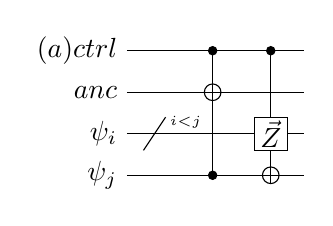
\begin{tikzpicture}[scale=1.000000,x=1pt,y=1pt]
\filldraw[color=white] (0.000000, -7.500000) rectangle (64.000000, 52.500000);
% Drawing wires
% Line 1: ctrl W \text{(a) }ctrl
\draw[color=black] (0.000000,45.000000) -- (64.000000,45.000000);
\draw[color=black] (0.000000,45.000000) node[left] {$\text{(a) }ctrl$};
% Line 2: anc W anc
\draw[color=black] (0.000000,30.000000) -- (64.000000,30.000000);
\draw[color=black] (0.000000,30.000000) node[left] {$anc$};
% Line 3: i W \psi_i
\draw[color=black] (0.000000,15.000000) -- (64.000000,15.000000);
\draw[color=black] (0.000000,15.000000) node[left] {$\psi_i$};
% Line 4: j W \psi_j
\draw[color=black] (0.000000,0.000000) -- (64.000000,0.000000);
\draw[color=black] (0.000000,0.000000) node[left] {$\psi_j$};
% Done with wires; drawing gates
% Line 6: i / ^{i<j}
\draw (6.000000, 9.000000) -- (14.000000, 21.000000);
\draw (12.000000, 18.000000) node[right] {$\scriptstyle{^{i<j}}$};
% Line 7: ctrl anc i j LABEL width=-10
% Line 8: ctrl j +anc
\draw (31.000000,45.000000) -- (31.000000,0.000000);
\filldraw (31.000000, 45.000000) circle(1.500000pt);
\filldraw (31.000000, 0.000000) circle(1.500000pt);
\begin{scope}
\draw[fill=white] (31.000000, 30.000000) circle(3.000000pt);
\clip (31.000000, 30.000000) circle(3.000000pt);
\draw (28.000000, 30.000000) -- (34.000000, 30.000000);
\draw (31.000000, 27.000000) -- (31.000000, 33.000000);
\end{scope}
% Line 10: i G $\vec{Z}$ ctrl +j
\draw (52.000000,45.000000) -- (52.000000,0.000000);
\begin{scope}
\draw[fill=white] (52.000000, 15.000000) +(-45.000000:8.485281pt and 8.485281pt) -- +(45.000000:8.485281pt and 8.485281pt) -- +(135.000000:8.485281pt and 8.485281pt) -- +(225.000000:8.485281pt and 8.485281pt) -- cycle;
\clip (52.000000, 15.000000) +(-45.000000:8.485281pt and 8.485281pt) -- +(45.000000:8.485281pt and 8.485281pt) -- +(135.000000:8.485281pt and 8.485281pt) -- +(225.000000:8.485281pt and 8.485281pt) -- cycle;
\draw (52.000000, 15.000000) node {$\vec{Z}$};
\end{scope}
\filldraw (52.000000, 45.000000) circle(1.500000pt);
\begin{scope}
\draw[fill=white] (52.000000, 0.000000) circle(3.000000pt);
\clip (52.000000, 0.000000) circle(3.000000pt);
\draw (49.000000, 0.000000) -- (55.000000, 0.000000);
\draw (52.000000, -3.000000) -- (52.000000, 3.000000);
\end{scope}
% Done with gates; drawing ending labels
% Done with ending labels; drawing cut lines and comments
% Done with comments
\end{tikzpicture}

        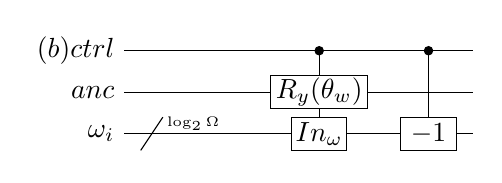
\begin{tikzpicture}[scale=1.000000,x=1pt,y=1pt]
\filldraw[color=white] (0.000000, -7.500000) rectangle (126.000000, 37.500000);
% Drawing wires
% Line 1: ctrl W \text{(b) }ctrl
\draw[color=black] (0.000000,30.000000) -- (126.000000,30.000000);
\draw[color=black] (0.000000,30.000000) node[left] {$\text{(b) }ctrl$};
% Line 2: anc W anc
\draw[color=black] (0.000000,15.000000) -- (126.000000,15.000000);
\draw[color=black] (0.000000,15.000000) node[left] {$anc$};
% Line 3: i W \omega_i
\draw[color=black] (0.000000,0.000000) -- (126.000000,0.000000);
\draw[color=black] (0.000000,0.000000) node[left] {$\omega_i$};
% Done with wires; drawing gates
% Line 5: i / ^{\log_2{\Omega}}
\draw (6.000000, -6.000000) -- (14.000000, 6.000000);
\draw (12.000000, 3.000000) node[right] {$\scriptstyle{^{\log_2{\Omega}}}$};
% Line 6: ctrl anc i LABEL
% Line 8: anc G:width=35 $R_y(\theta_w)$ i G:width=20 $In_\omega$ ctrl
\draw (70.500000,30.000000) -- (70.500000,0.000000);
\begin{scope}
\draw[fill=white] (70.500000, 15.000000) +(-45.000000:24.748737pt and 8.485281pt) -- +(45.000000:24.748737pt and 8.485281pt) -- +(135.000000:24.748737pt and 8.485281pt) -- +(225.000000:24.748737pt and 8.485281pt) -- cycle;
\clip (70.500000, 15.000000) +(-45.000000:24.748737pt and 8.485281pt) -- +(45.000000:24.748737pt and 8.485281pt) -- +(135.000000:24.748737pt and 8.485281pt) -- +(225.000000:24.748737pt and 8.485281pt) -- cycle;
\draw (70.500000, 15.000000) node {$R_y(\theta_w)$};
\end{scope}
\begin{scope}
\draw[fill=white] (70.500000, -0.000000) +(-45.000000:14.142136pt and 8.485281pt) -- +(45.000000:14.142136pt and 8.485281pt) -- +(135.000000:14.142136pt and 8.485281pt) -- +(225.000000:14.142136pt and 8.485281pt) -- cycle;
\clip (70.500000, -0.000000) +(-45.000000:14.142136pt and 8.485281pt) -- +(45.000000:14.142136pt and 8.485281pt) -- +(135.000000:14.142136pt and 8.485281pt) -- +(225.000000:14.142136pt and 8.485281pt) -- cycle;
\draw (70.500000, -0.000000) node {$In_\omega$};
\end{scope}
\filldraw (70.500000, 30.000000) circle(1.500000pt);
% Line 9: i G width=20 $-1$ ctrl
\draw (110.000000,30.000000) -- (110.000000,0.000000);
\begin{scope}
\draw[fill=white] (110.000000, -0.000000) +(-45.000000:14.142136pt and 8.485281pt) -- +(45.000000:14.142136pt and 8.485281pt) -- +(135.000000:14.142136pt and 8.485281pt) -- +(225.000000:14.142136pt and 8.485281pt) -- cycle;
\clip (110.000000, -0.000000) +(-45.000000:14.142136pt and 8.485281pt) -- +(45.000000:14.142136pt and 8.485281pt) -- +(135.000000:14.142136pt and 8.485281pt) -- +(225.000000:14.142136pt and 8.485281pt) -- cycle;
\draw (110.000000, -0.000000) node {$-1$};
\end{scope}
\filldraw (110.000000, 30.000000) circle(1.500000pt);
% Done with gates; drawing ending labels
% Done with ending labels; drawing cut lines and comments
% Done with comments
\end{tikzpicture}

    }
    \caption{
        \textbf{Bosonic Ladder Operator Block-Encoding}
        In subfigure a, a block-encoding for the bosonic creation operator, $a_i^\dagger$, is given.
        In subfigure b, a block-encoding for the bosonic annihilation operator, $a_i$, is given.
    }
    \label{fig:bosonic-ladder-op-be}
\end{figure}

The desired action of the block-encoding circuit for the bosonic creation operator is to increase the occupation of the bosonic mode by $1$ and rotate the block-encoding ancilla such that it has a coefficient of $\sqrt{\frac{\omega_i + 1}{\Omega}}$ in the $\ket{0}$ state when the occupation of the $i^\text{th}$ bosonic mode is $w_i$ prior to the operation.
This can be achieved by applying an incrementer circuit to the register encoding the occupation of the bosonic mode which increases the occupation by $1 \mod \Omega$ in each branch of the wavefunction.
The corresponding coefficients can be attained using a series of $R_y$ gates with different angles, controlled on the corresponding occupation state of the bosonic mode, and applied to the block-encoding ancilla.
An example circuit diagram for this circuit is given in subfigure \ref{fig:bosonic-ladder-op-be}a.
The angle of the $R_y$ gate can be classically determined by the following function:
\begin{equation}
    \label{eq:single-op-angles}
    \theta(\omega_i) = 
    \begin{cases} 
        2\sin^{-1}\Big(\sqrt{\frac{\omega_i}{\Omega}}\Big) & \text{when } \omega_i < \Omega\\
        0 & \text{when } \omega_i = \Omega
    \end{cases}
\end{equation}
where the choice of $\omega_i$ here in comparison with $\omega_i + 1$ in Eq. \ref{eq:be-bos-creation} is due to the occupation of the state being updated prior to these rotations.

A block-encoding circuit for the bosonic annihilation operator can be constructed similarly.
The only necessary modification is that the multiplexed rotations are applied prior to the incrementer circuit.
An example circuit diagram is given in subfigure \ref{fig:bosonic-ladder-op-be}b.

An implementation of a controlled incrementer circuit is given in \cite{Gidney_2015} which requires $\lceil \log_2\Omega \rceil$ Toffoli gates.
The series of controlled rotation gates can be implemented using a set of multiplexed rotations which can be decomposed via the protocol given in Möttönen et. al \cite{mottonen2004transformation}.
A discussion of different schemes to construct a \textit{controlled} set of multiplexed rotations is given in Appendix \ref{sec:multiplexed-rotations} and we opt for the decomposition that requires $\Omega$ uncontrolled rotations and $1$ controlled rotation.
A controlled rotation can be decomposed into $2$ uncontrolled rotations as shown in Figure \ref{fig:controlled-rotation}.
As a result, this block-encoding has a rescaling factor of $\sqrt{\Omega}$, requires one block-encoding ancilla, and uses $\lceil \log_2\Omega \rceil$ Toffoli gates and $\Omega + 2$ arbitrary rotations.


\subsection{Products of Bosonic Ladder Operators}

In this subsection, we discuss constructing block-encodings for a product of bosonic ladder operators acting on the same mode.

Unlike fermions, multiple bosons can occupy the same bosonic mode.
Therefore a bosonic ladder operator that is raised to an integer power can be applied to the state without necessarily zeroing-out the state.
Consider the desired action of a block-encoding for series of $R$ bosonic creation operators acting on the $i^\text{th}$ bosonic mode:
\begin{equation}
    \label{eq:be-S-creation-ops}
    U_{(a^\dagger_i)^R} \ket{\omega_i} \ket{0}_\text{anc} = 
    \begin{cases}
        \prod_{r=1}^{R} \sqrt{\frac{\omega_i + r}{\Omega}} \ket{\omega_i + R} \ket{0}_\text{anc} + \beta_\psi \ket{\perp} & \text{when } \omega_i \leq \Omega - R \\
        \ket{\perp} & \text{when } \omega_i > \Omega - R \\
    
    \end{cases}
\end{equation}

\begin{figure}
    \mbox{
        \include{figures/qpic-code/bosonic/products/R-creation}
        \include{figures/qpic-code/bosonic/products/S-annihilation}
    }
    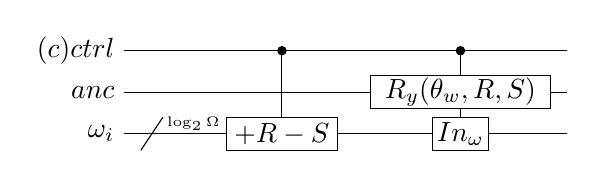
\begin{tikzpicture}[scale=1.000000,x=1pt,y=1pt]
\filldraw[color=white] (0.000000, -7.500000) rectangle (160.000000, 37.500000);
% Drawing wires
% Line 1: ctrl W \text{(c) }ctrl
\draw[color=black] (0.000000,30.000000) -- (160.000000,30.000000);
\draw[color=black] (0.000000,30.000000) node[left] {$\text{(c) }ctrl$};
% Line 2: anc W anc
\draw[color=black] (0.000000,15.000000) -- (160.000000,15.000000);
\draw[color=black] (0.000000,15.000000) node[left] {$anc$};
% Line 3: i W \omega_i
\draw[color=black] (0.000000,0.000000) -- (160.000000,0.000000);
\draw[color=black] (0.000000,0.000000) node[left] {$\omega_i$};
% Done with wires; drawing gates
% Line 5: i / ^{\log_2{\Omega}}
\draw (6.000000, -6.000000) -- (14.000000, 6.000000);
\draw (12.000000, 3.000000) node[right] {$\scriptstyle{^{\log_2{\Omega}}}$};
% Line 6: ctrl anc i LABEL width=-1
% Line 8: i G width=40 $+R-S$ ctrl
\draw (57.000000,30.000000) -- (57.000000,0.000000);
\begin{scope}
\draw[fill=white] (57.000000, -0.000000) +(-45.000000:28.284271pt and 8.485281pt) -- +(45.000000:28.284271pt and 8.485281pt) -- +(135.000000:28.284271pt and 8.485281pt) -- +(225.000000:28.284271pt and 8.485281pt) -- cycle;
\clip (57.000000, -0.000000) +(-45.000000:28.284271pt and 8.485281pt) -- +(45.000000:28.284271pt and 8.485281pt) -- +(135.000000:28.284271pt and 8.485281pt) -- +(225.000000:28.284271pt and 8.485281pt) -- cycle;
\draw (57.000000, -0.000000) node {$+R-S$};
\end{scope}
\filldraw (57.000000, 30.000000) circle(1.500000pt);
% Line 9: anc G:width=65 $R_y(\theta_w, R, S)$ i G:width=20 $In_\omega$ ctrl
\draw (121.500000,30.000000) -- (121.500000,0.000000);
\begin{scope}
\draw[fill=white] (121.500000, 15.000000) +(-45.000000:45.961941pt and 8.485281pt) -- +(45.000000:45.961941pt and 8.485281pt) -- +(135.000000:45.961941pt and 8.485281pt) -- +(225.000000:45.961941pt and 8.485281pt) -- cycle;
\clip (121.500000, 15.000000) +(-45.000000:45.961941pt and 8.485281pt) -- +(45.000000:45.961941pt and 8.485281pt) -- +(135.000000:45.961941pt and 8.485281pt) -- +(225.000000:45.961941pt and 8.485281pt) -- cycle;
\draw (121.500000, 15.000000) node {$R_y(\theta_w, R, S)$};
\end{scope}
\begin{scope}
\draw[fill=white] (121.500000, -0.000000) +(-45.000000:14.142136pt and 8.485281pt) -- +(45.000000:14.142136pt and 8.485281pt) -- +(135.000000:14.142136pt and 8.485281pt) -- +(225.000000:14.142136pt and 8.485281pt) -- cycle;
\clip (121.500000, -0.000000) +(-45.000000:14.142136pt and 8.485281pt) -- +(45.000000:14.142136pt and 8.485281pt) -- +(135.000000:14.142136pt and 8.485281pt) -- +(225.000000:14.142136pt and 8.485281pt) -- cycle;
\draw (121.500000, -0.000000) node {$In_\omega$};
\end{scope}
\filldraw (121.500000, 30.000000) circle(1.500000pt);
% Done with gates; drawing ending labels
% Done with ending labels; drawing cut lines and comments
% Done with comments
\end{tikzpicture}

    \caption{
        \textbf{Block-Encoding Product of Bosonic Ladder Operators}
        In subfigure a, a block-encoding for the operator $(a_i^\dagger)^R$ is given.
        In subfigure b, a block-encoding for the operator $(a_i)^S$ is given.
        In subfigure c, a block-encoding for the operator $(a_i^\dagger)^R (a_i)^S$ is given.
    }
    \label{fig:products-bosonic-operators}
\end{figure}

A block-encoding of this form could be achieved by simply repeating the construction for the individual bosonic creation operator (subfigure \ref{fig:bosonic-ladder-op-be}a) $R$ times.
However, a more efficient compilation can be achieved by updating the occupation of the bosonic mode by $+R$ and then performing a single series of controlled multiplexed rotations.
An example circuit diagram for this block-encoding is shown in subfigure \ref{fig:products-bosonic-operators}a.
The angles of the multiplexed rotations can be determined classically using the following function:
\begin{equation}
    \theta(\omega_i, R) = 
    \begin{cases} 
        2\sin^{-1}\Big(\prod_{r=0}^{R-1}\sqrt{\frac{\omega_i - r}{\Omega}}\Big) & \text{when } \omega_i \leq \Omega - R \\
        0 & \text{when } \omega_i > \Omega - R
    \end{cases}
\end{equation}
where the choice of $\omega_i - r$ here in comparison with $\omega_i + r$ in Eq. \ref{eq:be-S-creation-ops} is due to the occupation of the state being updated prior to these rotations.

A block-encoding for a bosonic annihilation operator being applied $S$ times can be achieved using a similar construction shown in subfigue \ref{fig:products-bosonic-operators}b.
The occupation of the mode is first decreased by $S$ and then the controlled multiplexed rotations are applied to pick up the corresponding coefficient on the block-encoding ancilla.
The function to determine the rotation angles is given by:
\begin{equation}
    \theta(\omega_i, S) = 
    \begin{cases} 
        2\sin^{-1}\Big(\prod_{s=1}^{S}\sqrt{\frac{\omega_i + s}{\Omega}}\Big) & \text{when } \omega_i \geq S \\
        0 & \text{when } \omega_i < S
    \end{cases}
\end{equation}

Likewise, we can construct a block-encoding for an operator of the form $(a_i^\dagger)^R (a_i)^S$ using a similar construction shown in subfigue \ref{fig:products-bosonic-operators}c.
The occupation of the mode is updated by a value of $+ R - S$ and then the controlled multiplexed rotations are applied to pick up the corresponding coefficient on the block-encoding ancilla.
The function to determine the rotation angles is given by:
\begin{equation}
    \theta(\omega_i, R, S) = 
    \begin{cases} 
        2\sin^{-1}\Big(\prod_{r=0}^{R-1}\sqrt{\frac{\omega_i - r}{\Omega}} \prod_{s=1}^{S}\sqrt{\frac{\omega_i - R + s}{\Omega}}\Big) & \text{when } S \leq \omega_i \leq \Omega - R \\
        0 & \text{Otherwise} 
    \end{cases}
\end{equation}

Incrementing a quantum register by a classical value can be implemented in multiple ways with different compilations having different space-time tradeoffs.
In this work, we often choose decompositions that reduce the number of non-Clifford operations at the expense or requiring more temporary ancillae, therefore we opt for the compilation given in Figure \ref{fig:addition-gate-efficient}.
This circuit requires, at most, $\lceil \log_2 \Omega \rceil - 1$ pairs of left and right elbows.
These block-encoding circuits have a rescaling factor of $\lambda = \Omega^{R+S/2}$, require one block-encoding ancilla, and use \textit{at most} $\Omega + \lceil \log_2 \Omega \rceil$ pairs of elbows and $\Omega + 2$ arbitrary rotations.


\subsection{Linear Combinations of Bosonic Ladder Operators}

In this subsection, we discuss constructing block-encodings for a linear combination of a product of bosonic ladder operators acting on the same mode plus its hermitian conjugate.

For a simple example, consider the operator $a_i^\dagger + a_i$.
Trivially, one could construct an LCO block-encoding by performing a linear combination of the block-encodings of the creation and annihilation operators respectively.
This block-encoding would have a rescaling factor of $\lambda = 2\sqrt{\Omega}$, use two block-encoding ancilla, and require $2\big(\lceil \log_2 \Omega \rceil - 1\big)$ pairs of elbows and $2 \big(\Omega + 2\big)$ arbitrary rotations.


\begin{figure}
    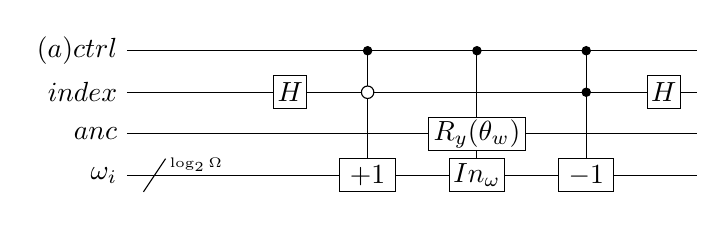
\begin{tikzpicture}[scale=1.000000,x=1pt,y=1pt]
\filldraw[color=white] (0.000000, -7.500000) rectangle (206.000000, 52.500000);
% Drawing wires
% Line 1: ctrl W \text{(a) }ctrl
\draw[color=black] (0.000000,45.000000) -- (206.000000,45.000000);
\draw[color=black] (0.000000,45.000000) node[left] {$\text{(a) }ctrl$};
% Line 2: index W index
\draw[color=black] (0.000000,30.000000) -- (206.000000,30.000000);
\draw[color=black] (0.000000,30.000000) node[left] {$index$};
% Line 3: anc W anc
\draw[color=black] (0.000000,15.000000) -- (206.000000,15.000000);
\draw[color=black] (0.000000,15.000000) node[left] {$anc$};
% Line 4: i W \omega_i
\draw[color=black] (0.000000,0.000000) -- (206.000000,0.000000);
\draw[color=black] (0.000000,0.000000) node[left] {$\omega_i$};
% Done with wires; drawing gates
% Line 6: i / ^{\log_2{\Omega}}
\draw (6.000000, -6.000000) -- (14.000000, 6.000000);
\draw (12.000000, 3.000000) node[right] {$\scriptstyle{^{\log_2{\Omega}}}$};
% Line 7: ctrl anc index i LABEL
% Line 9: index G $H$
\begin{scope}
\draw[fill=white] (59.000000, 30.000000) +(-45.000000:8.485281pt and 8.485281pt) -- +(45.000000:8.485281pt and 8.485281pt) -- +(135.000000:8.485281pt and 8.485281pt) -- +(225.000000:8.485281pt and 8.485281pt) -- cycle;
\clip (59.000000, 30.000000) +(-45.000000:8.485281pt and 8.485281pt) -- +(45.000000:8.485281pt and 8.485281pt) -- +(135.000000:8.485281pt and 8.485281pt) -- +(225.000000:8.485281pt and 8.485281pt) -- cycle;
\draw (59.000000, 30.000000) node {$H$};
\end{scope}
% Line 10: i G width=20 $+1$ ctrl -index
\draw (87.000000,45.000000) -- (87.000000,0.000000);
\begin{scope}
\draw[fill=white] (87.000000, -0.000000) +(-45.000000:14.142136pt and 8.485281pt) -- +(45.000000:14.142136pt and 8.485281pt) -- +(135.000000:14.142136pt and 8.485281pt) -- +(225.000000:14.142136pt and 8.485281pt) -- cycle;
\clip (87.000000, -0.000000) +(-45.000000:14.142136pt and 8.485281pt) -- +(45.000000:14.142136pt and 8.485281pt) -- +(135.000000:14.142136pt and 8.485281pt) -- +(225.000000:14.142136pt and 8.485281pt) -- cycle;
\draw (87.000000, -0.000000) node {$+1$};
\end{scope}
\filldraw (87.000000, 45.000000) circle(1.500000pt);
\draw[fill=white] (87.000000, 30.000000) circle(2.250000pt);
% Line 11: anc G:width=35 $R_y(\theta_w)$ i G:width=20 $In_\omega$ ctrl
\draw (126.500000,45.000000) -- (126.500000,0.000000);
\begin{scope}
\draw[fill=white] (126.500000, 15.000000) +(-45.000000:24.748737pt and 8.485281pt) -- +(45.000000:24.748737pt and 8.485281pt) -- +(135.000000:24.748737pt and 8.485281pt) -- +(225.000000:24.748737pt and 8.485281pt) -- cycle;
\clip (126.500000, 15.000000) +(-45.000000:24.748737pt and 8.485281pt) -- +(45.000000:24.748737pt and 8.485281pt) -- +(135.000000:24.748737pt and 8.485281pt) -- +(225.000000:24.748737pt and 8.485281pt) -- cycle;
\draw (126.500000, 15.000000) node {$R_y(\theta_w)$};
\end{scope}
\begin{scope}
\draw[fill=white] (126.500000, -0.000000) +(-45.000000:14.142136pt and 8.485281pt) -- +(45.000000:14.142136pt and 8.485281pt) -- +(135.000000:14.142136pt and 8.485281pt) -- +(225.000000:14.142136pt and 8.485281pt) -- cycle;
\clip (126.500000, -0.000000) +(-45.000000:14.142136pt and 8.485281pt) -- +(45.000000:14.142136pt and 8.485281pt) -- +(135.000000:14.142136pt and 8.485281pt) -- +(225.000000:14.142136pt and 8.485281pt) -- cycle;
\draw (126.500000, -0.000000) node {$In_\omega$};
\end{scope}
\filldraw (126.500000, 45.000000) circle(1.500000pt);
% Line 12: i G width=20 $-1$ ctrl index
\draw (166.000000,45.000000) -- (166.000000,0.000000);
\begin{scope}
\draw[fill=white] (166.000000, -0.000000) +(-45.000000:14.142136pt and 8.485281pt) -- +(45.000000:14.142136pt and 8.485281pt) -- +(135.000000:14.142136pt and 8.485281pt) -- +(225.000000:14.142136pt and 8.485281pt) -- cycle;
\clip (166.000000, -0.000000) +(-45.000000:14.142136pt and 8.485281pt) -- +(45.000000:14.142136pt and 8.485281pt) -- +(135.000000:14.142136pt and 8.485281pt) -- +(225.000000:14.142136pt and 8.485281pt) -- cycle;
\draw (166.000000, -0.000000) node {$-1$};
\end{scope}
\filldraw (166.000000, 45.000000) circle(1.500000pt);
\filldraw (166.000000, 30.000000) circle(1.500000pt);
% Line 13: index G $H$
\begin{scope}
\draw[fill=white] (194.000000, 30.000000) +(-45.000000:8.485281pt and 8.485281pt) -- +(45.000000:8.485281pt and 8.485281pt) -- +(135.000000:8.485281pt and 8.485281pt) -- +(225.000000:8.485281pt and 8.485281pt) -- cycle;
\clip (194.000000, 30.000000) +(-45.000000:8.485281pt and 8.485281pt) -- +(45.000000:8.485281pt and 8.485281pt) -- +(135.000000:8.485281pt and 8.485281pt) -- +(225.000000:8.485281pt and 8.485281pt) -- cycle;
\draw (194.000000, 30.000000) node {$H$};
\end{scope}
% Done with gates; drawing ending labels
% Done with ending labels; drawing cut lines and comments
% Done with comments
\end{tikzpicture}

    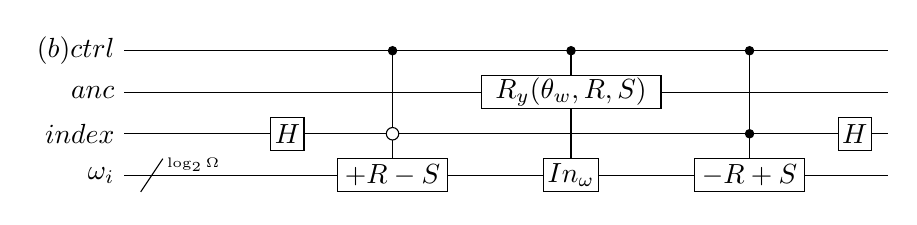
\begin{tikzpicture}[scale=1.000000,x=1pt,y=1pt]
\filldraw[color=white] (0.000000, -7.500000) rectangle (276.000000, 52.500000);
% Drawing wires
% Line 1: ctrl W \text{(b) }ctrl
\draw[color=black] (0.000000,45.000000) -- (276.000000,45.000000);
\draw[color=black] (0.000000,45.000000) node[left] {$\text{(b) }ctrl$};
% Line 2: anc W anc
\draw[color=black] (0.000000,30.000000) -- (276.000000,30.000000);
\draw[color=black] (0.000000,30.000000) node[left] {$anc$};
% Line 3: index W index
\draw[color=black] (0.000000,15.000000) -- (276.000000,15.000000);
\draw[color=black] (0.000000,15.000000) node[left] {$index$};
% Line 4: i W \omega_i
\draw[color=black] (0.000000,0.000000) -- (276.000000,0.000000);
\draw[color=black] (0.000000,0.000000) node[left] {$\omega_i$};
% Done with wires; drawing gates
% Line 6: i / ^{\log_2{\Omega}}
\draw (6.000000, -6.000000) -- (14.000000, 6.000000);
\draw (12.000000, 3.000000) node[right] {$\scriptstyle{^{\log_2{\Omega}}}$};
% Line 7: ctrl anc index i LABEL
% Line 9: index G $H$
\begin{scope}
\draw[fill=white] (59.000000, 15.000000) +(-45.000000:8.485281pt and 8.485281pt) -- +(45.000000:8.485281pt and 8.485281pt) -- +(135.000000:8.485281pt and 8.485281pt) -- +(225.000000:8.485281pt and 8.485281pt) -- cycle;
\clip (59.000000, 15.000000) +(-45.000000:8.485281pt and 8.485281pt) -- +(45.000000:8.485281pt and 8.485281pt) -- +(135.000000:8.485281pt and 8.485281pt) -- +(225.000000:8.485281pt and 8.485281pt) -- cycle;
\draw (59.000000, 15.000000) node {$H$};
\end{scope}
% Line 10: i G width=40 $+R-S$ ctrl -index
\draw (97.000000,45.000000) -- (97.000000,0.000000);
\begin{scope}
\draw[fill=white] (97.000000, -0.000000) +(-45.000000:28.284271pt and 8.485281pt) -- +(45.000000:28.284271pt and 8.485281pt) -- +(135.000000:28.284271pt and 8.485281pt) -- +(225.000000:28.284271pt and 8.485281pt) -- cycle;
\clip (97.000000, -0.000000) +(-45.000000:28.284271pt and 8.485281pt) -- +(45.000000:28.284271pt and 8.485281pt) -- +(135.000000:28.284271pt and 8.485281pt) -- +(225.000000:28.284271pt and 8.485281pt) -- cycle;
\draw (97.000000, -0.000000) node {$+R-S$};
\end{scope}
\filldraw (97.000000, 45.000000) circle(1.500000pt);
\draw[fill=white] (97.000000, 15.000000) circle(2.250000pt);
% Line 11: anc G:width=65 $R_y(\theta_w, R, S)$ i G:width=20 $In_\omega$ ctrl
\draw (161.500000,45.000000) -- (161.500000,0.000000);
\begin{scope}
\draw[fill=white] (161.500000, 30.000000) +(-45.000000:45.961941pt and 8.485281pt) -- +(45.000000:45.961941pt and 8.485281pt) -- +(135.000000:45.961941pt and 8.485281pt) -- +(225.000000:45.961941pt and 8.485281pt) -- cycle;
\clip (161.500000, 30.000000) +(-45.000000:45.961941pt and 8.485281pt) -- +(45.000000:45.961941pt and 8.485281pt) -- +(135.000000:45.961941pt and 8.485281pt) -- +(225.000000:45.961941pt and 8.485281pt) -- cycle;
\draw (161.500000, 30.000000) node {$R_y(\theta_w, R, S)$};
\end{scope}
\begin{scope}
\draw[fill=white] (161.500000, -0.000000) +(-45.000000:14.142136pt and 8.485281pt) -- +(45.000000:14.142136pt and 8.485281pt) -- +(135.000000:14.142136pt and 8.485281pt) -- +(225.000000:14.142136pt and 8.485281pt) -- cycle;
\clip (161.500000, -0.000000) +(-45.000000:14.142136pt and 8.485281pt) -- +(45.000000:14.142136pt and 8.485281pt) -- +(135.000000:14.142136pt and 8.485281pt) -- +(225.000000:14.142136pt and 8.485281pt) -- cycle;
\draw (161.500000, -0.000000) node {$In_\omega$};
\end{scope}
\filldraw (161.500000, 45.000000) circle(1.500000pt);
% Line 12: i G width=40 $-R+S$ ctrl index
\draw (226.000000,45.000000) -- (226.000000,0.000000);
\begin{scope}
\draw[fill=white] (226.000000, -0.000000) +(-45.000000:28.284271pt and 8.485281pt) -- +(45.000000:28.284271pt and 8.485281pt) -- +(135.000000:28.284271pt and 8.485281pt) -- +(225.000000:28.284271pt and 8.485281pt) -- cycle;
\clip (226.000000, -0.000000) +(-45.000000:28.284271pt and 8.485281pt) -- +(45.000000:28.284271pt and 8.485281pt) -- +(135.000000:28.284271pt and 8.485281pt) -- +(225.000000:28.284271pt and 8.485281pt) -- cycle;
\draw (226.000000, -0.000000) node {$-R+S$};
\end{scope}
\filldraw (226.000000, 45.000000) circle(1.500000pt);
\filldraw (226.000000, 15.000000) circle(1.500000pt);
% Line 13: index G $H$
\begin{scope}
\draw[fill=white] (264.000000, 15.000000) +(-45.000000:8.485281pt and 8.485281pt) -- +(45.000000:8.485281pt and 8.485281pt) -- +(135.000000:8.485281pt and 8.485281pt) -- +(225.000000:8.485281pt and 8.485281pt) -- cycle;
\clip (264.000000, 15.000000) +(-45.000000:8.485281pt and 8.485281pt) -- +(45.000000:8.485281pt and 8.485281pt) -- +(135.000000:8.485281pt and 8.485281pt) -- +(225.000000:8.485281pt and 8.485281pt) -- cycle;
\draw (264.000000, 15.000000) node {$H$};
\end{scope}
% Done with gates; drawing ending labels
% Done with ending labels; drawing cut lines and comments
% Done with comments
\end{tikzpicture}

    \caption{
        \textbf{Block-Encoding Product of Bosonic Ladder Operators Plus Hermitian Conjugate}
        In subfigure a, a block-encoding for the operator $(a_i^\dagger + a_i)$ is given.
        In subfigure b, a block-encoding for the operator $\big((a_i^\dagger)^R (a_i)^S + (a_i^\dagger)^S (a_i)^R\big)$ is given.
    }
    \label{fig:lc-bosonic}
\end{figure}


Due to the symmetry of the block-encodings for the individual operators, we can produce a more gate-efficient compilation.
For the annihilation operator, we wish to decrease the occupancy by $1$ and then apply the rotations.
Whereas for the creation operator, we wish in apply the rotations and then increase the occupancy by $1$.
Since the desired rotation angles are independent of which operator is being applied (Eq. \ref{eq:single-op-angles}), we can reuse the multiplexed rotations to apply the appropriate angles for both terms.
An example circuit diagram for this block-encoding is shown in subfigue \ref{fig:lc-bosonic}a.
Similarly, a block-encoding for the generalized operator $\big((a_i^\dagger)^R (a_i)^S + (a_i^\dagger)^S (a_i)^R\big)$ can be constructed and is shown in subfigure \ref{fig:lc-bosonic}b.

This compilation strategy is chosen under the assumption that the cost of implementing the multiplexed rotations exceeds the cost of the incrementer circuit.
If the inverse were true, a compilation could be constructed where the incrementer circuit is reused for both terms and the multiplexed rotations would be applied twice.  

For these block-encoding circuits, one additional pair of elbows is required to index between the two controlled incrementer circuits in Figure \ref{fig:lc-bosonic}.
Therefore, these block-encodings have a rescaling factor of $\lambda = 2 \Omega^{R+S/2}$, use two block-encoding ancilla, and require $\Omega + 2\big(\lceil \log_2 \Omega \rceil\big)$ pairs of elbows and $\Omega + 2$ arbitrary rotations.

\subsection{Terms with Fermionic and Bosonic Ladder Operators}

In the previous subsections, we discussed strategies for compiling block-encodings of different products and linear combinations of ladder operators acting on either fermionic or bosonic modes.
In this subsection, we discuss how to generate block-encodings for operators that contain both fermionic and bosonic operators.

\begin{figure}
    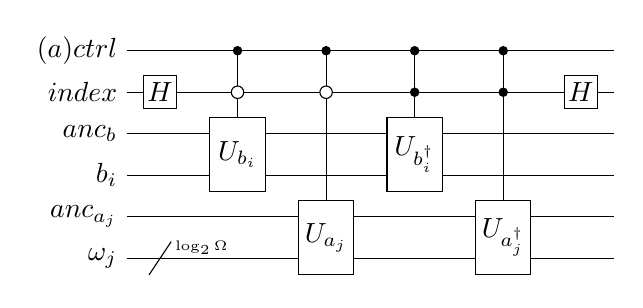
\begin{tikzpicture}[scale=1.000000,x=1pt,y=1pt]
\filldraw[color=white] (0.000000, -7.500000) rectangle (176.000000, 82.500000);
% Drawing wires
% Line 1: ctrl W \text{(a) }ctrl
\draw[color=black] (0.000000,75.000000) -- (176.000000,75.000000);
\draw[color=black] (0.000000,75.000000) node[left] {$\text{(a) }ctrl$};
% Line 2: index W index
\draw[color=black] (0.000000,60.000000) -- (176.000000,60.000000);
\draw[color=black] (0.000000,60.000000) node[left] {$index$};
% Line 3: anc_b W anc_b
\draw[color=black] (0.000000,45.000000) -- (176.000000,45.000000);
\draw[color=black] (0.000000,45.000000) node[left] {$anc_b$};
% Line 4: i W b_i
\draw[color=black] (0.000000,30.000000) -- (176.000000,30.000000);
\draw[color=black] (0.000000,30.000000) node[left] {$b_i$};
% Line 5: anc_a W anc_{a_j}
\draw[color=black] (0.000000,15.000000) -- (176.000000,15.000000);
\draw[color=black] (0.000000,15.000000) node[left] {$anc_{a_j}$};
% Line 6: j W \omega_j
\draw[color=black] (0.000000,0.000000) -- (176.000000,0.000000);
\draw[color=black] (0.000000,0.000000) node[left] {$\omega_j$};
% Done with wires; drawing gates
% Line 8: j / ^{\log_2{\Omega}}
\draw (8.000000, -6.000000) -- (16.000000, 6.000000);
\draw (14.000000, 3.000000) node[right] {$\scriptstyle{^{\log_2{\Omega}}}$};
% Line 10: index G $H$
\begin{scope}
\draw[fill=white] (12.000000, 60.000000) +(-45.000000:8.485281pt and 8.485281pt) -- +(45.000000:8.485281pt and 8.485281pt) -- +(135.000000:8.485281pt and 8.485281pt) -- +(225.000000:8.485281pt and 8.485281pt) -- cycle;
\clip (12.000000, 60.000000) +(-45.000000:8.485281pt and 8.485281pt) -- +(45.000000:8.485281pt and 8.485281pt) -- +(135.000000:8.485281pt and 8.485281pt) -- +(225.000000:8.485281pt and 8.485281pt) -- cycle;
\draw (12.000000, 60.000000) node {$H$};
\end{scope}
% Line 11: i anc_b G width=20 $U_{b_i}$ ctrl -index
\draw (40.000000,75.000000) -- (40.000000,30.000000);
\begin{scope}
\draw[fill=white] (40.000000, 37.500000) +(-45.000000:14.142136pt and 19.091883pt) -- +(45.000000:14.142136pt and 19.091883pt) -- +(135.000000:14.142136pt and 19.091883pt) -- +(225.000000:14.142136pt and 19.091883pt) -- cycle;
\clip (40.000000, 37.500000) +(-45.000000:14.142136pt and 19.091883pt) -- +(45.000000:14.142136pt and 19.091883pt) -- +(135.000000:14.142136pt and 19.091883pt) -- +(225.000000:14.142136pt and 19.091883pt) -- cycle;
\draw (40.000000, 37.500000) node {$U_{b_i}$};
\end{scope}
\filldraw (40.000000, 75.000000) circle(1.500000pt);
\draw[fill=white] (40.000000, 60.000000) circle(2.250000pt);
% Line 12: j anc_a G width=20 $U_{a_j}$ ctrl -index
\draw (72.000000,75.000000) -- (72.000000,0.000000);
\begin{scope}
\draw[fill=white] (72.000000, 7.500000) +(-45.000000:14.142136pt and 19.091883pt) -- +(45.000000:14.142136pt and 19.091883pt) -- +(135.000000:14.142136pt and 19.091883pt) -- +(225.000000:14.142136pt and 19.091883pt) -- cycle;
\clip (72.000000, 7.500000) +(-45.000000:14.142136pt and 19.091883pt) -- +(45.000000:14.142136pt and 19.091883pt) -- +(135.000000:14.142136pt and 19.091883pt) -- +(225.000000:14.142136pt and 19.091883pt) -- cycle;
\draw (72.000000, 7.500000) node {$U_{a_j}$};
\end{scope}
\filldraw (72.000000, 75.000000) circle(1.500000pt);
\draw[fill=white] (72.000000, 60.000000) circle(2.250000pt);
% Line 13: i anc_b G width=20 $U_{b_i^\dagger}$ ctrl index
\draw (104.000000,75.000000) -- (104.000000,30.000000);
\begin{scope}
\draw[fill=white] (104.000000, 37.500000) +(-45.000000:14.142136pt and 19.091883pt) -- +(45.000000:14.142136pt and 19.091883pt) -- +(135.000000:14.142136pt and 19.091883pt) -- +(225.000000:14.142136pt and 19.091883pt) -- cycle;
\clip (104.000000, 37.500000) +(-45.000000:14.142136pt and 19.091883pt) -- +(45.000000:14.142136pt and 19.091883pt) -- +(135.000000:14.142136pt and 19.091883pt) -- +(225.000000:14.142136pt and 19.091883pt) -- cycle;
\draw (104.000000, 37.500000) node {$U_{b_i^\dagger}$};
\end{scope}
\filldraw (104.000000, 75.000000) circle(1.500000pt);
\filldraw (104.000000, 60.000000) circle(1.500000pt);
% Line 14: j anc_a G width=20 $U_{a_j^\dagger}$ ctrl index
\draw (136.000000,75.000000) -- (136.000000,0.000000);
\begin{scope}
\draw[fill=white] (136.000000, 7.500000) +(-45.000000:14.142136pt and 19.091883pt) -- +(45.000000:14.142136pt and 19.091883pt) -- +(135.000000:14.142136pt and 19.091883pt) -- +(225.000000:14.142136pt and 19.091883pt) -- cycle;
\clip (136.000000, 7.500000) +(-45.000000:14.142136pt and 19.091883pt) -- +(45.000000:14.142136pt and 19.091883pt) -- +(135.000000:14.142136pt and 19.091883pt) -- +(225.000000:14.142136pt and 19.091883pt) -- cycle;
\draw (136.000000, 7.500000) node {$U_{a_j^\dagger}$};
\end{scope}
\filldraw (136.000000, 75.000000) circle(1.500000pt);
\filldraw (136.000000, 60.000000) circle(1.500000pt);
% Line 15: index G $H$
\begin{scope}
\draw[fill=white] (164.000000, 60.000000) +(-45.000000:8.485281pt and 8.485281pt) -- +(45.000000:8.485281pt and 8.485281pt) -- +(135.000000:8.485281pt and 8.485281pt) -- +(225.000000:8.485281pt and 8.485281pt) -- cycle;
\clip (164.000000, 60.000000) +(-45.000000:8.485281pt and 8.485281pt) -- +(45.000000:8.485281pt and 8.485281pt) -- +(135.000000:8.485281pt and 8.485281pt) -- +(225.000000:8.485281pt and 8.485281pt) -- cycle;
\draw (164.000000, 60.000000) node {$H$};
\end{scope}
% Done with gates; drawing ending labels
% Done with ending labels; drawing cut lines and comments
% Done with comments
\end{tikzpicture}

    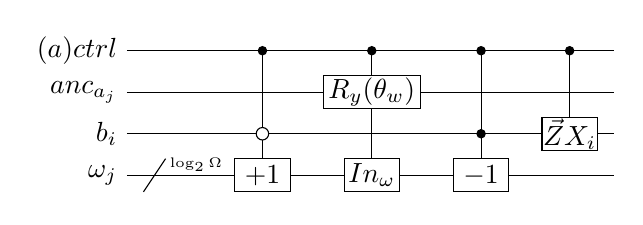
\begin{tikzpicture}[scale=1.000000,x=1pt,y=1pt]
\filldraw[color=white] (0.000000, -7.500000) rectangle (176.000000, 52.500000);
% Drawing wires
% Line 1: ctrl W \text{(a) }ctrl
\draw[color=black] (0.000000,45.000000) -- (176.000000,45.000000);
\draw[color=black] (0.000000,45.000000) node[left] {$\text{(a) }ctrl$};
% Line 2: anc_a W anc_{a_j}
\draw[color=black] (0.000000,30.000000) -- (176.000000,30.000000);
\draw[color=black] (0.000000,30.000000) node[left] {$anc_{a_j}$};
% Line 3: i W b_i
\draw[color=black] (0.000000,15.000000) -- (176.000000,15.000000);
\draw[color=black] (0.000000,15.000000) node[left] {$b_i$};
% Line 4: j W \omega_j
\draw[color=black] (0.000000,0.000000) -- (176.000000,0.000000);
\draw[color=black] (0.000000,0.000000) node[left] {$\omega_j$};
% Done with wires; drawing gates
% Line 6: j / ^{\log_2{\Omega}}
\draw (6.000000, -6.000000) -- (14.000000, 6.000000);
\draw (12.000000, 3.000000) node[right] {$\scriptstyle{^{\log_2{\Omega}}}$};
% Line 7: ctrl i anc_a j LABEL width=1
% Line 9: j G width=20 $+1$ ctrl -i
\draw (49.000000,45.000000) -- (49.000000,0.000000);
\begin{scope}
\draw[fill=white] (49.000000, -0.000000) +(-45.000000:14.142136pt and 8.485281pt) -- +(45.000000:14.142136pt and 8.485281pt) -- +(135.000000:14.142136pt and 8.485281pt) -- +(225.000000:14.142136pt and 8.485281pt) -- cycle;
\clip (49.000000, -0.000000) +(-45.000000:14.142136pt and 8.485281pt) -- +(45.000000:14.142136pt and 8.485281pt) -- +(135.000000:14.142136pt and 8.485281pt) -- +(225.000000:14.142136pt and 8.485281pt) -- cycle;
\draw (49.000000, -0.000000) node {$+1$};
\end{scope}
\filldraw (49.000000, 45.000000) circle(1.500000pt);
\draw[fill=white] (49.000000, 15.000000) circle(2.250000pt);
% Line 10: anc_a G:width=35 $R_y(\theta_w)$ j G:width=20 $In_\omega$ ctrl
\draw (88.500000,45.000000) -- (88.500000,0.000000);
\begin{scope}
\draw[fill=white] (88.500000, 30.000000) +(-45.000000:24.748737pt and 8.485281pt) -- +(45.000000:24.748737pt and 8.485281pt) -- +(135.000000:24.748737pt and 8.485281pt) -- +(225.000000:24.748737pt and 8.485281pt) -- cycle;
\clip (88.500000, 30.000000) +(-45.000000:24.748737pt and 8.485281pt) -- +(45.000000:24.748737pt and 8.485281pt) -- +(135.000000:24.748737pt and 8.485281pt) -- +(225.000000:24.748737pt and 8.485281pt) -- cycle;
\draw (88.500000, 30.000000) node {$R_y(\theta_w)$};
\end{scope}
\begin{scope}
\draw[fill=white] (88.500000, -0.000000) +(-45.000000:14.142136pt and 8.485281pt) -- +(45.000000:14.142136pt and 8.485281pt) -- +(135.000000:14.142136pt and 8.485281pt) -- +(225.000000:14.142136pt and 8.485281pt) -- cycle;
\clip (88.500000, -0.000000) +(-45.000000:14.142136pt and 8.485281pt) -- +(45.000000:14.142136pt and 8.485281pt) -- +(135.000000:14.142136pt and 8.485281pt) -- +(225.000000:14.142136pt and 8.485281pt) -- cycle;
\draw (88.500000, -0.000000) node {$In_\omega$};
\end{scope}
\filldraw (88.500000, 45.000000) circle(1.500000pt);
% Line 11: j G width=20 $-1$ ctrl i
\draw (128.000000,45.000000) -- (128.000000,0.000000);
\begin{scope}
\draw[fill=white] (128.000000, -0.000000) +(-45.000000:14.142136pt and 8.485281pt) -- +(45.000000:14.142136pt and 8.485281pt) -- +(135.000000:14.142136pt and 8.485281pt) -- +(225.000000:14.142136pt and 8.485281pt) -- cycle;
\clip (128.000000, -0.000000) +(-45.000000:14.142136pt and 8.485281pt) -- +(45.000000:14.142136pt and 8.485281pt) -- +(135.000000:14.142136pt and 8.485281pt) -- +(225.000000:14.142136pt and 8.485281pt) -- cycle;
\draw (128.000000, -0.000000) node {$-1$};
\end{scope}
\filldraw (128.000000, 45.000000) circle(1.500000pt);
\filldraw (128.000000, 15.000000) circle(1.500000pt);
% Line 13: i G width=20 $\vec{Z}X_i$ ctrl
\draw (160.000000,45.000000) -- (160.000000,15.000000);
\begin{scope}
\draw[fill=white] (160.000000, 15.000000) +(-45.000000:14.142136pt and 8.485281pt) -- +(45.000000:14.142136pt and 8.485281pt) -- +(135.000000:14.142136pt and 8.485281pt) -- +(225.000000:14.142136pt and 8.485281pt) -- cycle;
\clip (160.000000, 15.000000) +(-45.000000:14.142136pt and 8.485281pt) -- +(45.000000:14.142136pt and 8.485281pt) -- +(135.000000:14.142136pt and 8.485281pt) -- +(225.000000:14.142136pt and 8.485281pt) -- cycle;
\draw (160.000000, 15.000000) node {$\vec{Z}X_i$};
\end{scope}
\filldraw (160.000000, 45.000000) circle(1.500000pt);
% Done with gates; drawing ending labels
% Done with ending labels; drawing cut lines and comments
% Done with comments
\end{tikzpicture}

    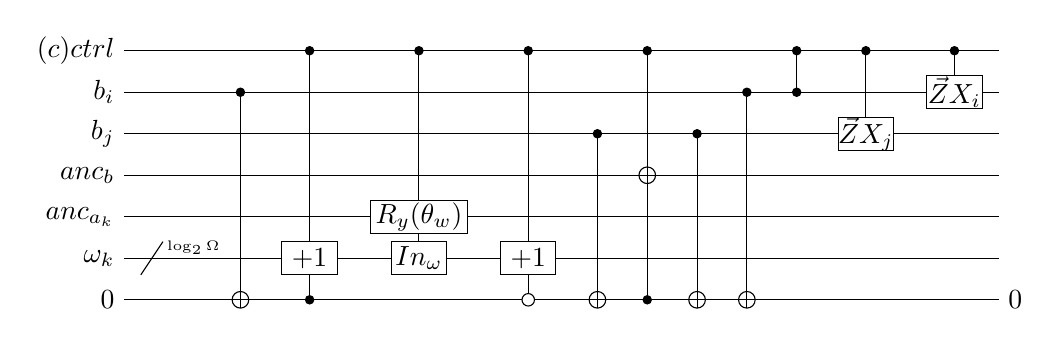
\begin{tikzpicture}[scale=1.000000,x=1pt,y=1pt]
\filldraw[color=white] (0.000000, -7.500000) rectangle (316.000000, 97.500000);
% Drawing wires
% Line 1: ctrl W \text{(c) }ctrl
\draw[color=black] (0.000000,90.000000) -- (316.000000,90.000000);
\draw[color=black] (0.000000,90.000000) node[left] {$\text{(c) }ctrl$};
% Line 2: i W b_i
\draw[color=black] (0.000000,75.000000) -- (316.000000,75.000000);
\draw[color=black] (0.000000,75.000000) node[left] {$b_i$};
% Line 3: j W b_j
\draw[color=black] (0.000000,60.000000) -- (316.000000,60.000000);
\draw[color=black] (0.000000,60.000000) node[left] {$b_j$};
% Line 4: anc_b W anc_b
\draw[color=black] (0.000000,45.000000) -- (316.000000,45.000000);
\draw[color=black] (0.000000,45.000000) node[left] {$anc_b$};
% Line 5: anc_a W anc_{a_k}
\draw[color=black] (0.000000,30.000000) -- (316.000000,30.000000);
\draw[color=black] (0.000000,30.000000) node[left] {$anc_{a_k}$};
% Line 6: k W \omega_k
\draw[color=black] (0.000000,15.000000) -- (316.000000,15.000000);
\draw[color=black] (0.000000,15.000000) node[left] {$\omega_k$};
% Line 7: c0 W 0 0
\draw[color=black] (0.000000,0.000000) -- (316.000000,0.000000);
\draw[color=black] (0.000000,0.000000) node[left] {$0$};
% Done with wires; drawing gates
% Line 9: k / ^{\log_2{\Omega}}
\draw (6.000000, 9.000000) -- (14.000000, 21.000000);
\draw (12.000000, 18.000000) node[right] {$\scriptstyle{^{\log_2{\Omega}}}$};
% Line 10: ctrl i j anc_b anc_a k c0 LABEL width=1
% Line 12: i +c0
\draw (42.000000,75.000000) -- (42.000000,0.000000);
\filldraw (42.000000, 75.000000) circle(1.500000pt);
\begin{scope}
\draw[fill=white] (42.000000, 0.000000) circle(3.000000pt);
\clip (42.000000, 0.000000) circle(3.000000pt);
\draw (39.000000, 0.000000) -- (45.000000, 0.000000);
\draw (42.000000, -3.000000) -- (42.000000, 3.000000);
\end{scope}
% Line 13: k G width=20 $+1$ ctrl c0
\draw (67.000000,90.000000) -- (67.000000,0.000000);
\begin{scope}
\draw[fill=white] (67.000000, 15.000000) +(-45.000000:14.142136pt and 8.485281pt) -- +(45.000000:14.142136pt and 8.485281pt) -- +(135.000000:14.142136pt and 8.485281pt) -- +(225.000000:14.142136pt and 8.485281pt) -- cycle;
\clip (67.000000, 15.000000) +(-45.000000:14.142136pt and 8.485281pt) -- +(45.000000:14.142136pt and 8.485281pt) -- +(135.000000:14.142136pt and 8.485281pt) -- +(225.000000:14.142136pt and 8.485281pt) -- cycle;
\draw (67.000000, 15.000000) node {$+1$};
\end{scope}
\filldraw (67.000000, 90.000000) circle(1.500000pt);
\filldraw (67.000000, 0.000000) circle(1.500000pt);
% Line 14: anc_a G:width=35 $R_y(\theta_w)$ k G:width=20 $In_\omega$ ctrl
\draw (106.500000,90.000000) -- (106.500000,15.000000);
\begin{scope}
\draw[fill=white] (106.500000, 30.000000) +(-45.000000:24.748737pt and 8.485281pt) -- +(45.000000:24.748737pt and 8.485281pt) -- +(135.000000:24.748737pt and 8.485281pt) -- +(225.000000:24.748737pt and 8.485281pt) -- cycle;
\clip (106.500000, 30.000000) +(-45.000000:24.748737pt and 8.485281pt) -- +(45.000000:24.748737pt and 8.485281pt) -- +(135.000000:24.748737pt and 8.485281pt) -- +(225.000000:24.748737pt and 8.485281pt) -- cycle;
\draw (106.500000, 30.000000) node {$R_y(\theta_w)$};
\end{scope}
\begin{scope}
\draw[fill=white] (106.500000, 15.000000) +(-45.000000:14.142136pt and 8.485281pt) -- +(45.000000:14.142136pt and 8.485281pt) -- +(135.000000:14.142136pt and 8.485281pt) -- +(225.000000:14.142136pt and 8.485281pt) -- cycle;
\clip (106.500000, 15.000000) +(-45.000000:14.142136pt and 8.485281pt) -- +(45.000000:14.142136pt and 8.485281pt) -- +(135.000000:14.142136pt and 8.485281pt) -- +(225.000000:14.142136pt and 8.485281pt) -- cycle;
\draw (106.500000, 15.000000) node {$In_\omega$};
\end{scope}
\filldraw (106.500000, 90.000000) circle(1.500000pt);
% Line 15: k G width=20 $+1$ ctrl -c0
\draw (146.000000,90.000000) -- (146.000000,0.000000);
\begin{scope}
\draw[fill=white] (146.000000, 15.000000) +(-45.000000:14.142136pt and 8.485281pt) -- +(45.000000:14.142136pt and 8.485281pt) -- +(135.000000:14.142136pt and 8.485281pt) -- +(225.000000:14.142136pt and 8.485281pt) -- cycle;
\clip (146.000000, 15.000000) +(-45.000000:14.142136pt and 8.485281pt) -- +(45.000000:14.142136pt and 8.485281pt) -- +(135.000000:14.142136pt and 8.485281pt) -- +(225.000000:14.142136pt and 8.485281pt) -- cycle;
\draw (146.000000, 15.000000) node {$+1$};
\end{scope}
\filldraw (146.000000, 90.000000) circle(1.500000pt);
\draw[fill=white] (146.000000, 0.000000) circle(2.250000pt);
% Line 16: j +c0
\draw (171.000000,60.000000) -- (171.000000,0.000000);
\filldraw (171.000000, 60.000000) circle(1.500000pt);
\begin{scope}
\draw[fill=white] (171.000000, 0.000000) circle(3.000000pt);
\clip (171.000000, 0.000000) circle(3.000000pt);
\draw (168.000000, 0.000000) -- (174.000000, 0.000000);
\draw (171.000000, -3.000000) -- (171.000000, 3.000000);
\end{scope}
% Line 18: ctrl c0 +anc_b
\draw (189.000000,90.000000) -- (189.000000,0.000000);
\filldraw (189.000000, 90.000000) circle(1.500000pt);
\filldraw (189.000000, 0.000000) circle(1.500000pt);
\begin{scope}
\draw[fill=white] (189.000000, 45.000000) circle(3.000000pt);
\clip (189.000000, 45.000000) circle(3.000000pt);
\draw (186.000000, 45.000000) -- (192.000000, 45.000000);
\draw (189.000000, 42.000000) -- (189.000000, 48.000000);
\end{scope}
% Line 19: j +c0
\draw (207.000000,60.000000) -- (207.000000,0.000000);
\filldraw (207.000000, 60.000000) circle(1.500000pt);
\begin{scope}
\draw[fill=white] (207.000000, 0.000000) circle(3.000000pt);
\clip (207.000000, 0.000000) circle(3.000000pt);
\draw (204.000000, 0.000000) -- (210.000000, 0.000000);
\draw (207.000000, -3.000000) -- (207.000000, 3.000000);
\end{scope}
% Line 20: i +c0
\draw (225.000000,75.000000) -- (225.000000,0.000000);
\filldraw (225.000000, 75.000000) circle(1.500000pt);
\begin{scope}
\draw[fill=white] (225.000000, 0.000000) circle(3.000000pt);
\clip (225.000000, 0.000000) circle(3.000000pt);
\draw (222.000000, 0.000000) -- (228.000000, 0.000000);
\draw (225.000000, -3.000000) -- (225.000000, 3.000000);
\end{scope}
% Line 22: ctrl i
\draw (243.000000,90.000000) -- (243.000000,75.000000);
\filldraw (243.000000, 90.000000) circle(1.500000pt);
\filldraw (243.000000, 75.000000) circle(1.500000pt);
% Line 24: j G width=20 $\vec{Z}X_j$ ctrl
\draw (268.000000,90.000000) -- (268.000000,60.000000);
\begin{scope}
\draw[fill=white] (268.000000, 60.000000) +(-45.000000:14.142136pt and 8.485281pt) -- +(45.000000:14.142136pt and 8.485281pt) -- +(135.000000:14.142136pt and 8.485281pt) -- +(225.000000:14.142136pt and 8.485281pt) -- cycle;
\clip (268.000000, 60.000000) +(-45.000000:14.142136pt and 8.485281pt) -- +(45.000000:14.142136pt and 8.485281pt) -- +(135.000000:14.142136pt and 8.485281pt) -- +(225.000000:14.142136pt and 8.485281pt) -- cycle;
\draw (268.000000, 60.000000) node {$\vec{Z}X_j$};
\end{scope}
\filldraw (268.000000, 90.000000) circle(1.500000pt);
% Line 25: i G width=20 $\vec{Z}X_i$ ctrl
\draw (300.000000,90.000000) -- (300.000000,75.000000);
\begin{scope}
\draw[fill=white] (300.000000, 75.000000) +(-45.000000:14.142136pt and 8.485281pt) -- +(45.000000:14.142136pt and 8.485281pt) -- +(135.000000:14.142136pt and 8.485281pt) -- +(225.000000:14.142136pt and 8.485281pt) -- cycle;
\clip (300.000000, 75.000000) +(-45.000000:14.142136pt and 8.485281pt) -- +(45.000000:14.142136pt and 8.485281pt) -- +(135.000000:14.142136pt and 8.485281pt) -- +(225.000000:14.142136pt and 8.485281pt) -- cycle;
\draw (300.000000, 75.000000) node {$\vec{Z}X_i$};
\end{scope}
\filldraw (300.000000, 90.000000) circle(1.500000pt);
% Done with gates; drawing ending labels
\draw[color=black] (316.000000,0.000000) node[right] {$0$};
% Done with ending labels; drawing cut lines and comments
% Done with comments
\end{tikzpicture}

    \caption{
        \textbf{Block-Encoding Terms}
        In subfigure a, a naive block-encoding for the operator $b_i a_j + a_j^\dagger b_i^\dagger$ is given.
        In subfigure b, a block-encoding for the operator $\big((a_i^\dagger)^R (a_i)^S + (a_i^\dagger)^S (a_i)^R\big)$ is given.
    }
    \label{fig:be-term-example}
\end{figure}


As an example, consider the operator: $b_i a_j + a_j^\dagger b_i^\dagger$.
Using Theorems \ref{th:product} and \ref{th:lco} to construct block-encodings of the individual terms and then combining them together would have a rescaling factor of $\lambda = 2*\sqrt{\Omega}$ and use $3$ block-encoding ancillae.
Additionally, the non-Clifford gate-cost would be $3$ Toffoli gates, 2 controlled incrementers, and $2*\Omega$ arbitrary rotations.
A circuit diagram for this construction is given in subfigure \ref{fig:be-term-example}a.

However, we can instead block-encode the entire operator at once by noting the action of the conjoined operator on the different occupation states of the fermionic mode.
Using the circuit shown in subfigure \ref{fig:be-term-example}b, the occupation of the fermionic mode is used to determine which bosonic operator is applied to the bosonic mode.
If the fermionic mode is occupied, then the bosonic annihilation operator is applied to apply the term $b_i a_j$.
If the fermionic mode is unoccupied, then the bosonic creation operator is applied to apply the term $b_i^\dagger a_j^\dagger$.
This block-encoding will have a rescaling factor of $\lambda = \sqrt{\Omega}$, use $1$ block-encoding ancillae, and require $1$ Toffoli gate, $2$ controlled incrementers, and $\Omega$ arbitrary rotations.

This strategy can be employed for other combinations of bosonic and fermionic ladder operators.
In the full Yukawa model, the operator $b_i b_j a_k^\dagger + b_j^\dagger b_i^\dagger a_k$ is used to describe the process of a fermion and antifermion being annihilated to form a boson as well as a boson being annihilated to form a fermion and antifermion.
For this operator, the occupation of either mode can be used to dictate which bosonic operator is applied to the system.
If both modes are occupied, then the bosonic creation operator should be applied.
If both modes are unoccupied, then the bosonic annihilation operator should be applied.
If the occupation of the two modes are not the same, then the state will be zeroed-out and the block-encoding ancilla for the fermionic modes will be flipped outside of the encoded subspace, therefore the action performed on the bosonic state will not matter.
A circuit diagram for this block-encoding is shown in subfigure \ref{fig:be-term-example}c.
This block-encoding has a rescaling factor of $\lambda = \sqrt{\Omega}$, uses $2$ block-encoding ancillae, and requires $2$ Toffolis, $2$ controlled incrementers, and $\Omega$ arbitrary rotations.


